\documentclass[a4paper,11pt,titlepage]{book}
\usepackage{amssymb}
\usepackage{fancyvrb,color,palatino}
\definecolor{gray}{gray}{0.6}


\newif\ifpdf
\ifx\pdfoutput\undefined
\pdffalse % es wird kein PDFLaTeX benutzt
\else
\pdfoutput=1 % es wird PDFLaTeX benutzt
\pdftrue
\fi

\ifpdf
\usepackage[pdftex]{graphicx}
\else
\usepackage{graphicx}
\fi

\upshape
\frenchspacing
\title{BKNR Manual}
\author{BKNR}

\begin{document}

\begin{titlepage}
\begin{center}

  \vspace*{6cm}
  \begin{figure}[htbp]
    \centering
    
\includegraphics[scale=0.6]{bknrlogo}
  \end{figure}
  \vspace{2cm}
  \Large
  CODENAME: SPUTNIK

\end{center}
\end{titlepage}

\tableofcontents

\chapter{Introduction}
\label{sec:introduction}

\vbox{
\centering
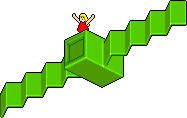
\includegraphics{satelliteicon}
\vspace{1cm}
}

BKNR is a software launch platform for Lisp satellites. You could
replace ``launch platform'' with framework and ``satellites'' with
``applications'', but that would be too many buzzwords.

BKNR is made of facilities that are not very useful on their own, but
they can be used to quickly build shiny and elegant Lisp
satellites. For example, a very important component of BKNR is its
datastore, which brings persistence to CLOS in a very simple way. By
adding a few declarations to your class definitions, you can have
persistent objects. You can also add XML import/export to your objects
in a similar way. I think this is the single most attractive feature
of BKNR: no more mapping from a relational database to Lisp objects,
no more XML parsing and XML generation, you just write plain
application code.


Another interesting feature of BKNR is its web framework, built on top
of the Hunchentoot webserver. The web framework has a simple
object-oriented handler hierarchy, with sessions, authorization and
all the features you are used to from other frameworks. It also
gathers usage information, stores it in the datastore, generates
statistics, maps sessions to persistent users. Furthermore, a very
useful feature is the HTML templater, which enables you to call Lisp
code from XML templates. The Lisp template callbacks are simple Lisp
functions that can work on the XML DOM representation. This eases
working with web developers, who can still use their standard editors
to develop the layout of the webpage. Dynamic content is easy to
integrate.

\begin{figure}[htbp]
    \centering
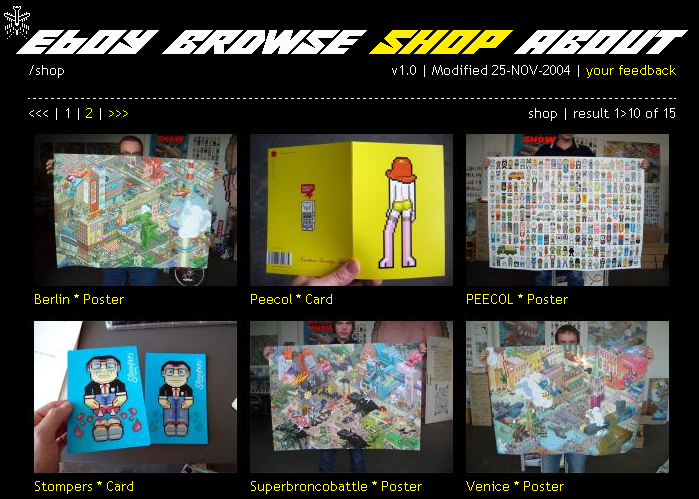
\includegraphics[scale=0.4]{eboyshot1}
\caption{Screenshot of eboy.com}
\end{figure}

The application which started BKNR was the website for the graphic
designers eboy. A lot of work went into the manipulation of images and
the integration of images into the Lisp framework. So another big part
of the BKNR web framework is the image manipulation code and the image
layout code, based on the CL-GD library by Edi Weitz.

We have started developing BKNR in March 2004, and it is used in 2 big
web applications (the Eboy dynasite ``eboy.com'', and the BOS website
``BOS creates rainforest''), and has been used to implement a few
personal websites (the website for the hacker gathering GPN in 2004,
which featured an interactive Lisp music-dj, the temporary conference
website for the European Lisp Workshop and the BKNR website). The code
was opensourced right from the start, but we didn't put a lot of
effort into making it accessible for other developers. This is the
first try at releasing some kind of public version of the BKNR
codebase, with (we hope) decent documentation.

If you would like to look at some of the BKNR features in a little
more detail, take the guided tour in Chapter 2. Chapters 3, 4, 5, 6
then show how to use the different facilities in short tutorials,
respectively object indices, the datastore, the web framework and the
templater. These chapters are slightly modified versions of the
tutorials that can be found in each of the facilities. Finally,
Chapter 7 shows how to build a full web photo album application using
BKNR. Due to time constraints, the last three chapters are not
available for the release of BKNR Sputnik. We are sorry for the
inconvenience. The sourcecode is in a working state, but not
documented and cleaned up yet.

We would like to thank the eboys for their support while developing
BKNR, their cool graphics and their enthusiasm :) We would also like
to thank Edi Weitz for his impressive libraries, and his
support. Also, I would like to thank Steffen Hurrle for his cool
website designs (he also has a new design for the BKNR website, which
sadly nobody has the time to update). The BKNR developers are Hans
Huebner, David Lichteblau and Manuel Odendahl.


\chapter{Guided Tour}

\vbox{
\centering

\includegraphics{guidedtouricon}
\vspace{1cm}
}

Let's take a guided tour of the BKNR sourcecode. Most facilities are
independent of each other, and can be used to build completely
different types of applications. However, all use the common toolbox
called `BKNR-UTILS', which contains a lot of small lisp
functions. These functions are not very important, and we will leave
them behind to get to the first important facility of the BKNR launch
platform.

\section{The Datastore}

The datastore is one of the oldest facilities in BKNR, its role is to
store the application data, so that this data is persistent between
LISP sessions. Most existing applications use a back-end
database to store persistent objects, for example a relational
database or an object-oriented database. Despite the immediate
advantages of having an existing database (reliability, speed,
management tools), this approach is quite cumbersome: every
application data structure has to be mapped onto a data structure in
the database. This is not trivial, as can be seen by the gazillions
attempts to write automatic conversion tools. Another fundamental
problem is the integration of the database into the language itself,
and into the development workflow. Errors in the database are
"external" to the LISP process, rollback, error-catching, transactions
are not as easy to write as they would be by having an "internal"
database. In the end, we believe that the advantages of having an
external database are outweighed by the disadvantages.

With the decreasing hardware costs nowadays, it is quite feasible for
most applications to keep their entire dataset in memory, and indeed
this is the approach taken by the BKNR datastore. Even with a growing
data set, memory costs decrease faster than the data grows, so that
evolution is not a problem. This approach is known as "prevalence",
and the BKNR datastore was initially based on the prevalence solution
by Sven Van Caekenberghe (also see
`http://homepage.mac.com/svc/prevalence/readme.html'). The key points
of the prevalence model are:

\begin{itemize}
\item All data is held in RAM

\item Changes to persistent data are written to a transaction log
   file. When loading the datastore, the transaction log is read, and
   all changes are applied to the persistent data. All changes ever
   made to the persistent data are executed in order, and the data is
   recovered.

\item If the data model supports it, the persistent data state can be
   captured and written to a file, which is called a "snapshot
   file". The snapshot file is read when loading the datastore, and
   the snapshotted data is used as a "starting point" for the
   transaction log.
\end{itemize}

In the datastore, transactions which are logged to the transaction log
are LISP functions defined using the `DEFTRANSACTION' form. Thus, all
transactions transforming persistent data are made explicit in the
source code. This if different from object-oriented databases, where
the fundamental transactions are object creation, object deletion and
slot access, which are not special cases in the prevalence model at
all. The main problem with this approach is that it is possible to
modify the persistent data in a way that is not logged into the
transaction log, which leads to lost data after reloading the
database. However, the BKNR datastore has a lot of development and
debugging helps, warning the user when he is making dangerous changes
(or forbidding them alltogether).

The datastore has gone through a few development iterations, which are
actually quite interesting to explain, as they show which compromises
have been made, and how the datastore can be tweaked. After having
used the prevalence solution of Sven van Caekenberghe and deciding
that it didn't quite fit our needs, we wrote a simple datastore
closely modelled on Sven's approach. However, the datastore featured
helpers to create and modify indexed CLOS objects. Also, the
transaction log consisted of SEXPs, and the loading of the transaction
log consisted of using the `LOAD' LISP function. The main part of the
object datastore consisted of a really big `DEFINE-PERSISTENT-CLASS'
macro, which generated a `DEFCLASS' form, and overrided a lot of
methods, making up a store generic method protocol. Special slot
options could be used to tell the store to index objects. For example,
you could specify that the slot `NAME' of the class `USER' was stored
in an index called `USER-NAME-INDEX'. The persistent objects could be
snapshotted and written to a snapshot file, which again was a LISP
file.

The main problem with this first approach was the lack of real CLOS
support. For example, you could modify an object using standard CLOS
methods like `SETF SLOT-VALUE' without ever getting a warning that
modifying the persistent state outside a transaction is
dangerous. Moreover, the `DEFINE-PERSISTENT-CLASS' macro was difficult
to modify, and the slot options for indices could not be modified
easily. This lead to the development of a separate index layer, a
separate transaction system, and of an object datastore combining the
two systems with additional CLOS support built using the Metaobject
Protocol.

\subsection{The transaction layer}

The transaction layer is now separate from the object oriented
datastore. It provides the functionality to declare explicit
transactions (still using the `DEFTRANSACTION' form), and to serialize
the transactions coming from multiple threads to a transaction log in
the filesystem. Using the transaction system is done by instantiating
an instance of the `STORE' class (or `MP-STORE' to serialize
concurrent transactions) and specifying a directory where the
transaction logs has to be stored. Only a single transaction system
can be open in a LISP session. When a transaction is executed, the
store serializes the transaction call (the transaction name and its
arguments) to the transaction log. It also stores the timestamp at
which the transaction was executed. This allows the user to restore
the transaction system state until a certain time (for debugging his
application or reverting to an old data state). When a datastore is
created or restored, the transaction log is read, and all the
transaction calls are re-executed. After all the transactions have
been executed, the persistent state is restored.

A transaction store can have multiple subsystems, which control a
certain subset of the persistent data. For example, the object
datastore which controls persistent CLOS objects is realized as a
subsystem of the transaction layer. A subsystem can snapshot the
current persistent state, and write it to disk. When the persistent
data is snapshotted, the transaction log can be discarded. Restoring
this state then consists of loading the snapshot file, and then
executing the transactions stored in the new transaction log. This
allows for a much faster restore procedure. The snapshotting procedure
takes care to backup the old transaction log, so that a restore until
a certain timestamp is still possible.

\subsection{The object datastore}

The object datastore combines several aspects:
\begin{itemize}
  \item It is a subsystem of the transaction layer, and can snapshot
persistent CLOS objects to a snapshot file, saving their slot values.
  \item It provides a CLOS Metaclass for persistent objects. Using
this metaclass, you can specify additional slot options for persistent
objects. For example, you can specify that a certain slot is
transient, which means that it will not be snapshotted and that its
value can be changed outside of a transaction.
  \item The persistent object metaclass also provides the index
facility of `BKNR-INDICES', so that persistent objects automatically
get indexed when restored from the store. The index facility is also
used by the store itself to keep track of the instantiated objects of
each class, and to index the objects by their unique ID.
\end{itemize}

The object datastore also provides a few helpers for developers. For
example, you cannot change the value of a slot when you are outside of
a transaction. The store throws an error when such an illegal
operation is made. The store also warns you when you change a class
definition. As the class definitions are not stored in the datastore,
a snapshot is necessary after schema evolution.

\section{The XML Import/Export Facility}

BKNR applications often have to communicate with the external world,
for example getting data from external sources, or exporting the data
from the object datastore to external sources. In order to reduce the
amount of conversion and parsing code that has to be written to
accomodate these tasks, the BKNR framework provides an automatic
mapping from CLOS classes to XML data. Using a special Metaclass for
XML objects, you can map a CLOS class to XML according to a XML
DTD.

In the following paragraphs, we will use the CLOS class `USER' to show
how the XML import/export facility works. The class `USER' has a slot
`PARENT' which points to another `USER', a slot `NAME' which contains
a string (the name of the user, obviously) and a slot `AGE' which
contains an integer (the age of the user).

A DTD consists of element declaration and of attribute declarations
(we will leave entity declarations aside for now). Most of the time,
the mapping between the XML data and the CLOS representation is quite
straightforward. An object is represented as an XML element, and its
slots are represented as either attributes of the element, or child
elements. All the data in the XML file is encoded as a string, and
read as such by the CXML parser used by BKNR. You can however specify
custom parsing and serializing routines for slots.

After the CLOS class has been annotated using specific slot-options,
objects can be read from an existing XML file (which validates against
the DTD file), or CLOS objects can be serialized to XML. Furthermore,
parent-child relations can be directly created by the parsing code, or
following by the serializing code. XML impex slot options can also be
combined with BKNR indices, which makes browsing XML data very simple.

Exporting and importing XML data now is a breeze!

\section{The BKNR Web Framework}

BKNR also features a web framework, providing an object oriented web
handler architecture. Adding handlers for special kinds of data (for
example RSS feeds for a custom data structure) can easily be achieved
using multiple inheritance. Furthermore, a template handler is
available, making it possible to access LISP functions from an XHTML
file. Sadly, as the web framework has been heavily rewritten in the
last months, we were not able to document it. However, you can have a
look at the example sourcecode for different applications on the bknr
webpage.


%\section{The Templater}


%\section{eboy.com}


\chapter{BKNR Indices}

\section{ Introduction}

In the framework we built as a backend for the `eboy.com' website,
we built a prevalence layer that could handle CLOS objects. These
CLOS objects all had an `ID', and could be indexed over other
slots as well. For example, we heavily used ``keyword indices'' that
could give back all objects that had a certain keyword stored in a
slot. However, the slot indices were built into a very big
`define-persistent-class' macro, and could not easily be extended
or used on their own.

This index layer is now built using the metaobject protocol, and
has a CLOS method protocol to access indices, so that new index
classes can easily be added.

This tutorial will show you how to create CLOS classes with slot
indices, class indices, and how to create custom indices and use
them with your classes.


\section{ Obtaining and loading BKNR slot indices}

You can obtain the current CVS sources of BKNR by following the
instructions at `http://bknr.net/blog/bknr-devel'. Add the `src'
directory of BKNR to your `asdf:*central-registry*', and load the
indices module by evaluating the following form:

\begin{Verbatim}[fontsize=\small,frame=leftline,framerule=0.9mm,rulecolor=\color{gray},framesep=5.1mm,xleftmargin=5mm,fontfamily=cmtt]
(asdf:oos 'asdf:load-op :bknr-indices)
\end{Verbatim}
Then switch to the `bknr.indices' package to try out the tutorial.

\begin{Verbatim}[fontsize=\small,frame=leftline,framerule=0.9mm,rulecolor=\color{gray},framesep=5.1mm,xleftmargin=5mm,fontfamily=cmtt]
(in-package :bknr.indices)
\end{Verbatim}


\section{ A simple indexed class}



\subsection{ A standard non-indexed class}

We begin by defining a simple class called GORILLA. Gorillas have
a name, and a description keyword.

\begin{Verbatim}[fontsize=\small,frame=leftline,framerule=0.9mm,rulecolor=\color{gray},framesep=5.1mm,xleftmargin=5mm,fontfamily=cmtt]
(defclass gorilla ()
  ((name        :initarg :name
      :reader gorilla-name
      :type string)
   (description :initarg :description
      :reader gorilla-description)))

(defmethod print-object ((gorilla gorilla) stream)
  (print-unreadable-object (gorilla stream :type t)
    (format stream "~S" (gorilla-name gorilla))))
\end{Verbatim}
We can create a few gorillas to test the class. To refer to these
gorillas later on, we have to store them in a list. We can then
write functions to search for gorillas.

\begin{Verbatim}[fontsize=\small,frame=leftline,framerule=0.9mm,rulecolor=\color{gray},framesep=5.1mm,xleftmargin=5mm,fontfamily=cmtt]
(defvar *gorillas* nil)

(setf *gorillas*
      (list
       (make-instance 'gorilla :name "Lucy"
            :description :aggressive)
       (make-instance 'gorilla :name "Robert"
            :description :playful)
       (make-instance 'gorilla :name "John"
            :description :aggressive)))

(defun all-gorillas ()
  (copy-list *gorillas*))

(defun gorilla-with-name (name)
  (find name *gorillas* :test #'string-equal
   :key #'gorilla-name))

(defun gorillas-with-description (description)
  (remove description *gorillas* :test-not #'eql :key
     #'gorilla-description))

(all-gorillas)
; => (#<GORILLA "Lucy"> #<GORILLA "Robert"> #<GORILLA "John">)
(gorilla-with-name "Lucy")
; => #<GORILLA "Lucy">
(gorillas-with-description :aggressive)
; => (#<GORILLA "Lucy"> #<GORILLA "John">)
(gorilla-with-name "Manuel")
; => NIL
\end{Verbatim}
What we would like to do however, is have the object system index
these objects for us. This is achieved by using INDEXED-CLASS as
the metaclass for the gorilla class. The `INDEXED-CLASS' has its
own slot-definition objects called `INDEX-DIRECT-SLOT-DEFINITION'
and `INDEX-EFFECTIVE-SLOT-DEFINITION'. Using these classes, we can
specify additional initargs to our slot definitions.



\subsection{ Additional slot initargs}

The following additional initargs are available:

`INDEX' - A class name that specifies the class of the index to
use. For example `SLOT-INDEX', `KEYWORD-INDEX' or
`KEYWORD-LIST-INDEX'.

`INDEX-INITARGS' - Additional arguments that are passed to
`INDEX-INITIALIZE' when creating the index.

`INDEX-READER' - A symbol under which a query function for the
index will be stored.

`INDEX-ALL' - A symbol under which a function returning all the
values of the index will be stored.

`INDEX-SUBCLASSES' - Determines if instances of subclasses of this
class will be indexed in the slot index also. Defaults to `T'.



\subsection{ A simple indexed class}

Using the `INDEXED-CLASS', we can redefine our gorilla example.

\begin{Verbatim}[fontsize=\small,frame=leftline,framerule=0.9mm,rulecolor=\color{gray},framesep=5.1mm,xleftmargin=5mm,fontfamily=cmtt]
(defclass gorilla ()
  ((name :initarg :name :reader gorilla-name
    :index-type slot-index
    :index-initargs (:test #'equal)
    :index-reader gorilla-with-name
    :index-values all-gorillas)
   (description :initarg :description
      :reader gorilla-description
      :index-type keyword-index
      :index-reader gorillas-with-description))
  (:metaclass indexed-class))
\end{Verbatim}
We have to recreate the gorillas though, as the old instances
don't get updated for now.

\begin{Verbatim}[fontsize=\small,frame=leftline,framerule=0.9mm,rulecolor=\color{gray},framesep=5.1mm,xleftmargin=5mm,fontfamily=cmtt]
(make-instance 'gorilla :name "Lucy" :description :aggressive)
(make-instance 'gorilla :name "Robert" :description :playful)
(make-instance 'gorilla :name "John" :description :aggressive)

(all-gorillas)
; => (#<GORILLA "Lucy"> #<GORILLA "Robert"> #<GORILLA "John">)
(gorilla-with-name "Lucy")
; => #<GORILLA "Lucy">
; T
(gorillas-with-description :aggressive)
; => (#<GORILLA "John"> #<GORILLA "Lucy">)
; T
\end{Verbatim}


\subsection{ Class indices}

We can also create indices that are not bound to a single
slot. These indices are called `CLASS-INDICES'. For example, we
can add two slots for the coordinates of the gorilla, and a class
index of type `ARRAY-INDEX' that will index the two slots `X' and
`Y' of the gorilla in an array of dimensions `256x256'. Note that
redefining the class conserves the existing indices.

\begin{Verbatim}[fontsize=\small,frame=leftline,framerule=0.9mm,rulecolor=\color{gray},framesep=5.1mm,xleftmargin=5mm,fontfamily=cmtt]
(defclass gorilla ()
  ((name :initarg :name :reader gorilla-name
    :index-type slot-index
    :index-initargs (:test #'equal)
    :index-reader gorilla-with-name
    :index-values all-gorillas)
   (description :initarg :description
      :reader gorilla-description
      :index-type keyword-index
      :index-reader gorillas-with-description)
   (x :initarg :x :reader gorilla-x)
   (y :initarg :y :reader gorilla-y))
  (:metaclass indexed-class)
  (:class-indices (coords :index-type array-index
           :slots (x y)
           :index-reader gorilla-with-coords
           :index-initargs (:dimensions '(256 256)))))

(make-instance 'gorilla :name "Pete" :description
          :playful :x 5 :y 8)

(gorilla-with-coords '(5 8))
; => #<GORILLA "Pete">
(all-gorillas)
; => (#<GORILLA "Lucy"> #<GORILLA "Robert">
;     #<GORILLA "John"> #<GORILLA "Pete">)
(gorillas-with-description :playful)
; => (#<GORILLA "Pete"> #<GORILLA "Robert">)
; T

(let ((lucy (gorilla-with-name "Lucy")))
  (with-slots (x y) lucy
    (setf x 0 y 0)))

(gorilla-with-name "Lucy")
; => #<GORILLA "Lucy">
; T
(gorilla-with-coords '(0 0))
; => #<GORILLA "Lucy">
\end{Verbatim}


\section{ Creating indexed classes}

Adding indexes to a class is very simple. The class has to have
the metaclass `INDEXED-CLASS', or a class deriving from
`INDEXED-CLASS'.



\subsection{ Slot indices}

`INDEXED-CLASS' uses its own `EFFECTIVE-SLOT-DEFINITION' and
`DIRECT-SLOT-DEFINITION' which add indices to slots. A slot
definition in the `DEFCLASS' form supports additional keyword
arguments:

`:INDEX' - Specifies an existing index to use as slot-index for this slot.

`:INDEX-TYPE' - Specifies the class of the index to be used for this
slot.

`:INDEX-INITARGS' - Specifies additional initargs to be given to
`INDEX-CREATE' when creating the index. The slot-name is given as
the `:SLOT' keyword argument to `INDEX-CREATE'.

`:INDEX-READER' - Specifies the name under which a query function
for the created index will be saved.

`:INDEX-VALUES' - Specifies the name under which a function returning
all the objects stored in the created index will be saved.

`:INDEX-MAPVALUES' - Specifies the name under which a function
applying a function to all the objects stored in the created index
will be saved.

`:INDEX-SUBCLASSES' - Specifies if subclasses of the class will
also be indexing in this index. Default is `T'.

For each `DIRECT-SLOT-DEFINITION' of an indexed class with the
`:INDEX' keyword, an index is created and stored in the
`DIRECT-SLOT-DEFINITION'. All the direct indexes are then stored
in the `EFFECTIVE-SLOT-DEFINITION' (indexes with
`INDEX-SUBCLASSES = NIL' will not).

Every access to the slot will update the indices stored in the
`EFFECTIVE-SLOT-DEFINITION'. When the slot is changed, the object
is removed from all the slot indices, and added after the slot
value has been changed. When a slot is made unbound, the object is
removed from the slot indices.

\begin{Verbatim}[fontsize=\small,frame=leftline,framerule=0.9mm,rulecolor=\color{gray},framesep=5.1mm,xleftmargin=5mm,fontfamily=cmtt]
(defclass test-slot ()
  ((a :initarg :a :index-type slot-index
      :reader test-slot-a
      :index-reader test-slot-with-a
      :index-values all-test-slots)
   (b :initarg :b :index-type slot-index
      :index-reader test-slot-with-b
      :index-subclasses nil
      :index-values all-test-slots-bs))
  (:metaclass indexed-class))

(defclass test-slot2 (test-slot)
  ((b :initarg :b :index-type slot-index
      :index-reader test-slot2-with-b
      :index-subclasses nil
      :index-mapvalues map-test-slot2s
      :index-values all-test-slot2s-bs))
  (:metaclass indexed-class))

(defmethod print-object ((object test-slot) stream)
  (print-unreadable-object (object stream :type t)
    (format stream "~S" (test-slot-a object))))

(make-instance 'test-slot :a 1 :b 2)
(make-instance 'test-slot :a 2 :b 3)
(make-instance 'test-slot2 :a 3 :b 4)
(make-instance 'test-slot2 :a 4 :b 2)
(make-instance 'test-slot2 :a 5 :b 9)

(all-test-slots)
; => (#<TEST-SLOT 1> #<TEST-SLOT 2> #<TEST-SLOT2 3>
;     #<TEST-SLOT2 4> #<TEST-SLOT2 5>)
(test-slot-with-a 2)
; => #<TEST-SLOT 2>
(all-test-slots-bs)
; => (#<TEST-SLOT 1> #<TEST-SLOT 2>)
(all-test-slot2s-bs)
; (#<TEST-SLOT2 3> #<TEST-SLOT2 4> #<TEST-SLOT2 5>)
(map-test-slot2s #'(lambda (obj) (print obj)))
; 
; #<TEST-SLOT2 3> 
; #<TEST-SLOT2 4> 
; #<TEST-SLOT2 5> 
; 
; NIL
\end{Verbatim}
Here is an example of a slot index using an already existing index.

\begin{Verbatim}[fontsize=\small,frame=leftline,framerule=0.9mm,rulecolor=\color{gray},framesep=5.1mm,xleftmargin=5mm,fontfamily=cmtt]
(defvar *existing-slot-index*
  (index-create 'slot-index :slots '(a)))

(defclass test-slot3 ()
  ((a :initarg :a :index *existing-slot-index*))
  (:metaclass indexed-class))

(make-instance 'test-slot3 :a 3)
(make-instance 'test-slot3 :a 4)

(index-get *existing-slot-index* 4)
; => #<TEST-SLOT3 {493B9655}>
; T
(index-values *existing-slot-index*)
; => (#<TEST-SLOT3 {493A0CBD}> #<TEST-SLOT3 {493B9655}>)
\end{Verbatim}
The slot indices of a class can be examined using
`CLASS-SLOT-INDICES'.

\begin{Verbatim}[fontsize=\small,frame=leftline,framerule=0.9mm,rulecolor=\color{gray},framesep=5.1mm,xleftmargin=5mm,fontfamily=cmtt]
(class-slot-indices (find-class 'test-slot) 'a)
; => (#<SLOT-INDEX SLOT: A SIZE: 5 {599FA9F5}>)
(class-slot-indices (find-class 'test-slot) 'b)
; => (#<SLOT-INDEX SLOT: B SIZE: 2 {59A038BD}>)
(class-slot-indices (find-class 'test-slot2) 'a)
; => (#<SLOT-INDEX SLOT: A SIZE: 5 {599FA9F5}>)
(class-slot-indices (find-class 'test-slot2) 'b)
; => (#<SLOT-INDEX SLOT: B SIZE: 3 {59A0D6A5}>)
\end{Verbatim}
Note that a slot can have multiple indices.

\begin{Verbatim}[fontsize=\small,frame=leftline,framerule=0.9mm,rulecolor=\color{gray},framesep=5.1mm,xleftmargin=5mm,fontfamily=cmtt]
(defclass test-slot4 (test-slot)
  ((a :initarg :a :index-type slot-index
      :index-reader test-slot4-with-a
      :index-values all-test-slot4s))
  (:metaclass indexed-class))

(make-instance 'test-slot4 :a 6 :b 9)

(all-test-slots)
; => (#<TEST-SLOT 1> #<TEST-SLOT 2> #<TEST-SLOT2 3>
;     #<TEST-SLOT2 4> #<TEST-SLOT2 5>
;     #<TEST-SLOT4 6>)
(all-test-slot4s)
; => (#<TEST-SLOT4 6>)
(class-slot-indices (find-class 'test-slot4) 'a)
; => (#<SLOT-INDEX SLOT: A SIZE: 6 {599FA9F5}>
;  #<SLOT-INDEX SLOT: A SIZE: 1 {59079E25}>)
\end{Verbatim}


\subsection{ Class indices}

In addition to slot indices, an indexed class supports class
indices which react when one of several slots is changing. For
example, in the `GORILLA' class above, the `COORDS' index reacts
on slots `X' and `Y'. By default, a class index reacts on all
slots.

A class index is created by adding a class option `CLASS-INDICES'
followed by a list of class index specifications.

\begin{Verbatim}[fontsize=\small,frame=leftline,framerule=0.9mm,rulecolor=\color{gray},framesep=5.1mm,xleftmargin=5mm,fontfamily=cmtt]
(defclass test-class ()
  ((x :initarg :x :reader test-class-x)
   (y :initarg :y :reader test-class-y)
   (z :initarg :z :reader test-class-z))
  (:metaclass indexed-class)
  (:class-indices (2d-coords :index-type array-index :slots (x y)
              :index-initargs (:dimensions '(256 256))
              :index-reader test-with-2d-coords)
        (3d-coords :index-type array-index :slots (x y z)
              :index-reader test-with-3d-coords
              :index-initargs (:dimensions '(256 256 2)))))

(defmethod print-object ((object test-class) stream)
  (print-unreadable-object (object stream :type t)
    (with-slots (x y z) object
      (format stream "~d,~d,~d" x y z))))

(make-instance 'test-class :x 1 :y 1 :z 0)
(make-instance 'test-class :x 1 :y 3 :z 1)
(make-instance 'test-class :x 1 :y 2 :z 0)

(test-with-3d-coords '(1 1 0))
; => #<TEST-CLASS 1,1,0>
(test-with-2d-coords '(1 1))
; => #<TEST-CLASS 1,1,0>
(test-with-2d-coords '(1 2))
; => #<TEST-CLASS 1,2,0>
\end{Verbatim}
A class index specification has to comply with the following
lambda-list `(NAME \&REST ARGS \&KEY INDEX-READER INDEX-VALUES SLOTS
TYPE INDEX \&ALLOW-OTHER-KEYS)'. The key arguments `:INDEX-TYPE',
`:INDEX', `:INDEX-READER' and `:INDEX-VALUES' are then removed from
the initargs, and the rest is passed to `INDEX-CREATE' to create
the class index.

`:INDEX-TYPE' - specifies the type of the class index.

`:INDEX' - (optional) specifies an already existing index object
to use.

`:INDEX-READER' - Like `:INDEX-READER' for slot
indices.

`:INDEX-VALUES' - Like `:INDEX-VALUES' for slot indices.

Using `:INDEX', we can use already existing indices as class
indices.

\begin{Verbatim}[fontsize=\small,frame=leftline,framerule=0.9mm,rulecolor=\color{gray},framesep=5.1mm,xleftmargin=5mm,fontfamily=cmtt]
(defvar *array-index*
  (index-create 'array-index :slots '(x y z)
      :dimensions '(256 256 2)))

(defclass test-class2 (test-class)
  ()
  (:metaclass indexed-class)
  (:class-indices (coords :index *array-index* :slots (x y z)
           :index-reader test-with-coords)))

(make-instance 'test-class2 :x 5 :y 5 :z 0)

*array-index*
; => #<ARRAY-INDEX SLOTS: (X Y Z) ((256 256 2)) {593F383D}>
(index-get *array-index* '( 5 5 0))
; => #<TEST-CLASS2 5,5,0>
(test-with-coords '(5 5 0))
; => #<TEST-CLASS2 5,5,0>
\end{Verbatim}
Another example of a class index is the `CLASS-INDEX' index.

\begin{Verbatim}[fontsize=\small,frame=leftline,framerule=0.9mm,rulecolor=\color{gray},framesep=5.1mm,xleftmargin=5mm,fontfamily=cmtt]
(defvar *class-index*
  (index-create 'class-index :index-subclasses t :slot-name 'id))
(defvar *object-id* 0)

(defclass base-object ()
  ((id :initform (incf *object-id*)))
  (:metaclass indexed-class)
  (:class-indices (class :index *class-index*
          :index-reader objects-of-class
          :index-values all-objects
          :index-subclasses t
          :index-keys all-class-names)
        (classes :index-type class-index
            :index-initargs (:index-superclasses t)
            :slots (id)
            :index-subclasses t
            :index-reader objects-with-class)))

(defclass child1 (base-object)
  ()
  (:metaclass indexed-class))

(defclass child2 (base-object)
  ((a :initarg :a))
  (:metaclass indexed-class))

(make-instance 'child1)
(make-instance 'child1)
(make-instance 'child1)
(make-instance 'child2)
(make-instance 'child2)

(all-objects)
; => (#<CHILD1 {48E5CB3D}> #<CHILD1 {48E51395}> #<CHILD1 {48E453DD}>
;  #<CHILD2 {48E82F55}> #<CHILD2 {48E7746D}>)
(objects-with-class 'child1)
; => (#<CHILD1 {48E5CB3D}> #<CHILD1 {48E51395}> #<CHILD1 {48E453DD}>)
; T
(objects-with-class 'child2)
; => (#<CHILD2 {48E82F55}> #<CHILD2 {48E7746D}>)
; T
(objects-with-class 'base-object)
; => (#<CHILD2 {48E82F55}> #<CHILD2 {48E7746D}> #<CHILD1 {48E5CB3D}>
;  #<CHILD1 {48E51395}> #<CHILD1 {48E453DD}>)
; T
(objects-of-class 'child1)
; => (#<CHILD1 {48E5CB3D}> #<CHILD1 {48E51395}> #<CHILD1 {48E453DD}>)
; T
(objects-of-class 'child2)
; => (#<CHILD2 {48E82F55}> #<CHILD2 {48E7746D}>)
; T
(objects-of-class 'base-object)
; => NIL
; NIL
\end{Verbatim}


\subsection{ Destroying objects}

Indexed objects will not be garbage collected until they are
removed from the indices. This is done by calling the
`DESTROY-OBJECT' method on the object. This removes the object
from all its indices, and sets the slot `DESTROYED-P' to `T', so
that not slot-access is possible anymore on the object.

\begin{Verbatim}[fontsize=\small,frame=leftline,framerule=0.9mm,rulecolor=\color{gray},framesep=5.1mm,xleftmargin=5mm,fontfamily=cmtt]
(let ((obj (test-with-coords '(5 5 0))))
       (destroy-object obj))
\end{Verbatim}
This will throw an error.


\begin{Verbatim}[fontsize=\small,frame=leftline,framerule=0.9mm,rulecolor=\color{gray},framesep=5.1mm,xleftmargin=5mm,fontfamily=cmtt]
(test-class-x obj)
\end{Verbatim}


\subsection{ Class and object reinitialization}

When a class is redefined, the indexed-class code tries to map
the new slot-indices to the old-indices. If it finds a slot-index
in the old `EFFECTIVE-SLOT-DEFINITION' and a slot-index in the new
`EFFECTIVE-SLOT-DEFINITION', it calls `INDEX-REINITIALIZE' on the
two indices to copy the values form the old index to the new
one. Afterwards, the same is done for the class
indices. `INDEX-REINITIALIZE' will not be called with the
old-index being the same as the new-index, so that explicitly
instantiated class indices don't get reinitialized with
themselves.

Indices for new slots or new class indices are obviously empty on
creation, and will be filled when the existing instances are
updated. For now, `SHARED-INITIALIZE' is not overloaded, so the
instance update are noticed through `(SETF SLOT-VALUE-USING-CLASS)'.


\section{ Creating a custom index}

The main reason to write indexed slots was to be able to use
custom indices that are appropriate for the task at hand. Indices
are CLOS objects that follow the index method protocol. The
methods that have to be implemented are:

`INDEX-ADD (INDEX OBJECT)' - Add OBJECT to the INDEX. Throws an
ERROR if a problem happened while inserting OBJECT."

`INDEX-GET (INDEX KEY)' - Get the object (or the objects) stored
under the index-key KEY.

`INDEX-REMOVE (INDEX OBJECT)' - Remove OBJECT from the INDEX.

`INDEX-KEYS (INDEX)' - Returns all the keys of the index.

`INDEX-VALUES (INDEX)' - Returns all the objects stored in INDEX.

`INDEX-REINITIALIZE (NEW-INDEX OLD-INDEX)' - Called when the
definition of an index is changed.

`INDEX-CLEAR (INDEX)' - Remove all indexed objects from the index.

In addition to this method, there is the function `INDEX-CREATE'
that instantiates an index object, and calls `INDEX-INITIALIZE' on
it.

The best way to see how this methods are used is to have at look
at the basic index `SLOT-INDEX'. A slot index indexes an object
under a key stored in a slot of this object, so a slot index is
initialized using two arguments: the slot-name where the key is
stored, and a test to create the underlying hash-table.

\begin{Verbatim}[fontsize=\small,frame=leftline,framerule=0.9mm,rulecolor=\color{gray},framesep=5.1mm,xleftmargin=5mm,fontfamily=cmtt]
(defclass slot-index ()
  ((hash-table :initarg :hash-table :accessor slot-index-hash-table
          :documentation "The internal hash table used to index
objects.")
   (slot-name :initarg :slot-name :reader slot-index-slot-name
         :documentation "The value of the slot with name
SLOT-NAME is used as a key to the internal hash-table.")
   (index-nil :initarg :index-nil :reader slot-index-index-nil
         :initform nil
         :documentation "If T, NIL is used as a valid slot
 value, else slots with NIL value are treated as unbound slots.")))

(defmethod initialize-instance :after
    ((index slot-index) &key (test #'eql) slots index-nil
     &allow-other-keys)
  (unless (<= (length slots) 1)
    (error "Can not create slot-index with more than one slot."))
  (with-slots (hash-table slot-name) index
    (setf hash-table (make-hash-table :test test)
     slot-name (first slots)
     (slot-value index 'index-nil) index-nil)))
\end{Verbatim}
When a class is redefined, the indices are re-created. However, we
still want our existing objects to be indexed by the new index,
therefore `INDEX-REINITIALIZE' copies the hash-table when the
hash-table test is the same, or else copies all the stored objects
into the new hash-table.

\begin{Verbatim}[fontsize=\small,frame=leftline,framerule=0.9mm,rulecolor=\color{gray},framesep=5.1mm,xleftmargin=5mm,fontfamily=cmtt]
(defmethod index-reinitialize ((new-index slot-index)
                (old-index slot-index))
  "Reinitialize the slot-bound index from the old index by copying the
internal hash-table if the hash-table test is the same, or by
iterating over the values of the old-table and reentering them into
the new hash-table."
  (let ((new-hash (slot-index-hash-table new-index))
   (old-hash (slot-index-hash-table old-index)))
    (if (eql (hash-table-test new-hash)
        (hash-table-test old-hash))
   (setf (slot-index-hash-table new-index)
         old-hash)
   (loop for key being the hash-keys of old-hash
         using (hash-value value)
         do (setf (gethash key new-hash) value)))
    new-index))
\end{Verbatim}
`INDEX-CLEAR' just creates an empty hash-table to replace the
existing hash-table.

\begin{Verbatim}[fontsize=\small,frame=leftline,framerule=0.9mm,rulecolor=\color{gray},framesep=5.1mm,xleftmargin=5mm,fontfamily=cmtt]
(defmethod index-clear ((index slot-index))
  (with-slots (hash-table) index
    (setf hash-table (make-hash-table
            :test (hash-table-test hash-table)))))
\end{Verbatim}
`INDEX-ADD' and `INDEX-REMOVE' both use the slot-name to get the
key value, and use this key to query the underlying
hash-table. When another object is stored under the key, an error
is thrown.

\begin{Verbatim}[fontsize=\small,frame=leftline,framerule=0.9mm,rulecolor=\color{gray},framesep=5.1mm,xleftmargin=5mm,fontfamily=cmtt]
(defmethod index-add ((index slot-index) object)
  "Add an object using the value of the specified slot as key.
When the hash-table entry already contains a value, an error
is thrown."
  (unless (slot-boundp object (slot-index-slot-name index))
    (return-from index-add))
  (let* ((key (slot-value object (slot-index-slot-name index)))
    (hash-table (slot-index-hash-table index)))
    (when (and (not (slot-index-index-nil index))
          (null key))
      (return-from index-add))
    (multiple-value-bind (value presentp)
   (gethash key hash-table)
      (when (and presentp
       (not (eql value object)))
   (error (make-condition 'index-existing-error
                :index index :key key :value value)))
      (setf (gethash key hash-table) object))))

(defmethod index-remove ((index slot-index) object)
  (let ((slot-name (slot-index-slot-name index)))
    (if (slot-boundp object slot-name)
   (remhash (slot-value object slot-name)
       (slot-index-hash-table index))
   (warn "Ignoring request to remove object ~a
with unbound slot ~A."
         object slot-name))))
\end{Verbatim}
The rest of the methods are straightforward.

\begin{Verbatim}[fontsize=\small,frame=leftline,framerule=0.9mm,rulecolor=\color{gray},framesep=5.1mm,xleftmargin=5mm,fontfamily=cmtt]
(defmethod index-get ((index slot-index) key)
  (gethash key (slot-index-hash-table index)))

(defmethod index-keys ((index slot-index))
  (loop for key being the hash-keys
   of (slot-index-hash-table index)
   collect key))

(defmethod index-values ((index slot-index))
  (loop for value being the hash-values
   of (slot-index-hash-table index)
   collect value))
\end{Verbatim}


\section{ Creating an index using multiple slots}

When creating an index using multiple slots, you have to take care
of a few things. It can happen that a slot-value used by the index
is updated, but that the other slots that are needed are
unbound. However, this is not always an error, so a class index
has to check that all the slots it needs are bound. This is the
`INDEX-ADD' method for an array index.

\begin{Verbatim}[fontsize=\small,frame=leftline,framerule=0.9mm,rulecolor=\color{gray},framesep=5.1mm,xleftmargin=5mm,fontfamily=cmtt]
(defmethod index-add ((index array-index) object)
  (let* ((slot-values
     (mapcar #'(lambda (slot-name)
            ;; return when not all slots are set
            ;;
            ;; - 18.10.04 not needed because of
            ;; make-instance around method
            ;;
            ;; - 19.10.04 in fact this is needed because
            ;; when adding a class index, the existing
            ;; instances are not reinitailized using
            ;; make-instnace, so we have to catch this...
            (unless (slot-boundp object slot-name)
                (return-from index-add nil))
              (slot-value object slot-name))
               (array-index-slot-names index)))
    (array (array-index-array index))
    (dimensions (array-dimensions array)))
    (loop for slot-value in slot-values
     for dimension in dimensions
     when (>= slot-value dimension)
     do (error "Could not add ~a to array-index ~a
because the coordinates ~a are out of bound."
          object index slot-values))
    (let ((value (apply #'aref array slot-values)))
      (when (and value
       (not (eql value object)))
   (error (make-condition 'index-existing-error
                :index index :key slot-values
                :value value))))
    (setf (apply #'aref array slot-values)
     object)))
\end{Verbatim}

\chapter{BKNR Datastore}

\vbox{
    \centering
    
\includegraphics{datastoreicon}
    \vspace{1cm}}

\section{ Introduction}



\subsection{ The prevalence model}

The BKNR datastore is a persistence solution for Lisp data. It
uses the prevalence model, which is based on the following
assumptions:

All data is held in RAM.

Data can be saved to disk at once into a snapshot file and is read
from that file at startup time.

Changes to persistent data are written to a transaction log file
immediately, which can be replayed to restore all changes that
occured since the last snapshot was saved.

Every kind of operation that needs to be logged is called a
``transaction'', and such transactions are made explicit in the
program code. This is different from object-oriented databases,
where the fundamental transactions are object creation, object
deletion and slot access, which are not special cases in the
prevalence model at all.

Isolation of transactions is achieved using thread locks. In the
simplest model used by the `mp-store', transactions are serialized
using a global lock.

The transaction system is responsible for providing replay of
committed transactions after a server crash, but not for rollback
of failed transactions in a running server, except that failing
transactions are simply not logged onto disk. To roll back
transactions at points where exceptions might be excepted, use
ordinary Lisp programming techniques involving `unwind-protect'
and similar.



\subsection{ BKNR Datastore Design}

The design of the datastore aims to make explicit the
orthogonality of object system access (unlogged) and logging of
transactions (essentially independent of the object system). The
interface between transaction system and object system is
documented and allows for the implementation of alternative object
systems. For example, the blob subsystem is using the same
interface as the object subsystem.

Previous versions of the BKNR Datastore allowed the creation of
multiple datastores in a single LISP process. However, this
feature was seldom used, and could be very confusing while
developing applications. The new version of the BKNR Datastore
supports only a single datastore, which is referenced by the
special variable `*STORE*'.



\subsection{ BKNR Object Datastore}

In addition to the transaction layer (in the file `txn.lisp'), the
BKNR datastore provides persistent CLOS objects using the
Metaobject Protocol. It provides a metaclass with which slots can
be defined as persistent (stored on snapshot) or transient. The
metaclass also prohibits slot accesses outside transactions,
provides unique IDs for all objects, and provides standard query
functions like `STORE-OBJECTS-WITH-CLASS' and
`STORE-OBJECTS-OF-CLASS'. The object datastore can be seamlessly
combined with BKNR indices and XML import/export.


\section{ Obtaining and loading BKNR Datastore}

You can obtain the current CVS sources of BKNR by following the
instructions at `http://bknr.net/blog/bknr-devel'. Add the `experimental'
directory of BKNR to your `asdf:*central-registry*', and load the
indices module by evaluating the following form:

\begin{Verbatim}[fontsize=\small,frame=leftline,framerule=0.9mm,rulecolor=\color{gray},framesep=5.1mm,xleftmargin=5mm,fontfamily=cmtt]
(asdf:oos 'asdf:load-op :bknr-datastore)
\end{Verbatim}
Then switch to the `bknr.datastore' package to try out the tutorial.

\begin{Verbatim}[fontsize=\small,frame=leftline,framerule=0.9mm,rulecolor=\color{gray},framesep=5.1mm,xleftmargin=5mm,fontfamily=cmtt]
(in-package :bknr.datastore)
\end{Verbatim}


\section{ A transaction system example}
The first datastore we will build is very simple. We have a
counter variable for the store, and this counter variable can be
decremented and indecremented. We want this variable to be
persistent, so decrementing and incrementing it has to be done
through transactions that will be logged by the datastore. We also
define a `:BEFORE' method for the generic function `RESTORE-STORE'
to set the counter to `0' initially. This method will be called
every time the store is created or restored from disk.

\begin{Verbatim}[fontsize=\small,frame=leftline,framerule=0.9mm,rulecolor=\color{gray},framesep=5.1mm,xleftmargin=5mm,fontfamily=cmtt]
(defclass tutorial-store (mp-store)
  ((counter :initform 0 :accessor tutorial-store-counter)))

(defmethod restore-store :before ((store tutorial-store) &key until)
  (declare (ignore until))
  (setf (tutorial-store-counter store) 0))
\end{Verbatim}
The two transactions are declared like normal functions, but using
the `DEFTRANSACTION' macro. 

\begin{Verbatim}[fontsize=\small,frame=leftline,framerule=0.9mm,rulecolor=\color{gray},framesep=5.1mm,xleftmargin=5mm,fontfamily=cmtt]
(deftransaction incf-counter ()
  (incf (tutorial-store-counter *store*)))

(deftransaction decf-counter ()
  (decf (tutorial-store-counter *store*)))
\end{Verbatim}
When looking at the macro-expanded form of `DEFTRANSACTION', we
see that `DEFTRANSACTION' defines two functions, a toplevel
function that creates a transaction object and calls the method
`EXECUTE' on it, and a function that contains the actual
transaction code and that will be called in the context of the
transaction, and logged to disk.

\begin{Verbatim}[fontsize=\small,frame=leftline,framerule=0.9mm,rulecolor=\color{gray},framesep=5.1mm,xleftmargin=5mm,fontfamily=cmtt]
(PROGN
 (DEFUN TX-DECF-COUNTER ()
   (UNLESS (IN-TRANSACTION-P) (ERROR 'NOT-IN-TRANSACTION))
   (DECF (TUTORIAL-STORE-COUNTER *STORE*)))
 (DEFUN DECF-COUNTER (&REST #:G3047)
   (EXECUTE
    (MAKE-INSTANCE 'TRANSACTION
                   :FUNCTION-SYMBOL
                   'TX-DECF-COUNTER
                   :TIMESTAMP
                   (GET-UNIVERSAL-TIME)
                   :ARGS
                   #:G3047))))
\end{Verbatim}
The new datastore only supports a single datastore instance per
LISP session. When creating a `STORE' object, the `*STORE*'
special variable is modified to point to the datastore. Thus, we
can create our simple datastore by creating an object of type
`TUTORIAL-STORE'. The transaction log will be store in the
directory ``/tmp/tutorial-store''.

\begin{Verbatim}[fontsize=\small,frame=leftline,framerule=0.9mm,rulecolor=\color{gray},framesep=5.1mm,xleftmargin=5mm,fontfamily=cmtt]
(make-instance 'tutorial-store :directory "/tmp/tutorial-store/"
          :subsystems nil)
; Warning:  restoring #<TUTORIAL-STORE DIR: "/tmp/tutorial-store/">
; => #<TUTORIAL-STORE DIR: "/tmp/tutorial-store/">

(tutorial-store-counter *store*)
; => 0
(incf-counter)
; => 1
(incf-counter)
; => 2
(decf-counter)
; => 1
\end{Verbatim}
The three transactions have been logged to the transaction log in
``/tmp/tutorial-store/'', as we can see:

\begin{Verbatim}[fontsize=\small,frame=leftline,framerule=0.9mm,rulecolor=\color{gray},framesep=5.1mm,xleftmargin=5mm,fontfamily=cmtt]
(with-open-file (s "/tmp/tutorial-store/current/transaction-log"
             :direction :input)
        (file-length s))
; => 126
(incf-counter)
; => 2
(with-open-file (s "/tmp/tutorial-store/current/transaction-log"
             :direction :input)
        (file-length s))
; => 168
\end{Verbatim}
The transaction log is kept in a directory called ``current'', which
is where the currently active version of the snapshots and log
files are kept. When a datastore is snapshotted, the ``current''
directory is backupped to another directory with the current date,
and snapshots are created in the new ``current'' directory. However,
we cannot snapshot our tutorial datastore, as we cannot snapshot
the persistent data (the counter value). 

\begin{Verbatim}[fontsize=\small,frame=leftline,framerule=0.9mm,rulecolor=\color{gray},framesep=5.1mm,xleftmargin=5mm,fontfamily=cmtt]
(snapshot)
; => Error in function (METHOD SNAPSHOT-STORE NIL (STORE)):
; => Cannot snapshot store without subsystems...
; => [Condition of type SIMPLE-ERROR]
\end{Verbatim}
We can close the store by using the function `CLOSE-STORE'.

\begin{Verbatim}[fontsize=\small,frame=leftline,framerule=0.9mm,rulecolor=\color{gray},framesep=5.1mm,xleftmargin=5mm,fontfamily=cmtt]
*store*
; => #<TUTORIAL-STORE DIR: "/tmp/tutorial-store/">
(close-store)
; => NIL
*store*
; => NIL
\end{Verbatim}
The store can then be recreated, and the transaction log will be
read and executed upon restore.

\begin{Verbatim}[fontsize=\small,frame=leftline,framerule=0.9mm,rulecolor=\color{gray},framesep=5.1mm,xleftmargin=5mm,fontfamily=cmtt]
(make-instance 'tutorial-store :directory "/tmp/tutorial-store/"
          :subsystems nil)

; Warning:  restoring #<TUTORIAL-STORE DIR: "/tmp/tutorial-store/">
; Warning:  loading transaction log
; /tmp/tutorial-store/current/transaction-log
; => #<TUTORIAL-STORE DIR: "/tmp/tutorial-store/">
(tutorial-store-counter *store*)
; => 2
\end{Verbatim}
The store can also be restored in a later LISP session. Make sure
that all the code necessary to the execution of the transaction
log has been loaded before restoring the datastore. A later
version of the datastore will log all the code necessary in the
datastore itself, so that code and data are synchronized.


\subsection{ Debugging the datastore}

By setting the `*STORE-DEBUG*' special variable to `T', the
datastore prints a lot of useful warnings. For example
You can also restore to a certain point in time, by specifying the
`UNTIL' argument of `RESTORE-STORE'.

\begin{Verbatim}[fontsize=\small,frame=leftline,framerule=0.9mm,rulecolor=\color{gray},framesep=5.1mm,xleftmargin=5mm,fontfamily=cmtt]
(setf *store-debug* t)
; => T
(restore-store *store*)
; Warning:  restoring #<TUTORIAL-STORE DIR: "/tmp/tutorial-store/">
; Warning:  loading transaction log
; /tmp/tutorial-store/current/transaction-log
; executing transaction #$(TX-INCF-COUNTER) at timestamp 3309258381
; executing transaction #$(TX-INCF-COUNTER) at timestamp 3309258383
; executing transaction #$(TX-DECF-COUNTER) at timestamp 3309258387
; executing transaction #$(TX-INCF-COUNTER) at timestamp 3309258390
; => :NORMAL
(tutorial-store-counter *store*)
; => 2
(restore-store *store* :until 3309258387)
; Warning:  restoring #<TUTORIAL-STORE DIR: "/tmp/tutorial-store/">
; Warning:  loading transaction log
; /tmp/tutorial-store/current/transaction-log
; executing transaction #$(TX-INCF-COUNTER) at timestamp 3309258381
; executing transaction #$(TX-INCF-COUNTER) at timestamp 3309258383
; executing transaction #$(TX-DECF-COUNTER) at timestamp 3309258387
; => :NORMAL
(tutorial-store-counter *store*)
; => 1
\end{Verbatim}


\subsection{ Adding a subsystem}
Now that we can restore the counter state by loading the
transaction log, we want to add a subsystem to be able to snapshot
the state of the counter. Thus, we won't need to execute every
single incrementing or decrementing transaction to restore our
persistent state.
To do this, we have to create a store-subsystem that will be able
to write the counter number to a file and to reload it on restore.

\begin{Verbatim}[fontsize=\small,frame=leftline,framerule=0.9mm,rulecolor=\color{gray},framesep=5.1mm,xleftmargin=5mm,fontfamily=cmtt]
(defclass counter-subsystem ()
  ())
\end{Verbatim}
Three methods are used to interact with the subsystem.
The first method is `INITIALIZE-SUBSYSTEM', which is called after
the store has been created and restored. It is used to initialize
certain parameters of the subsystem. We won't use this method
here, as our subsystem is very simple.
The second method is `SNAPSHOT-SUBSYSTEM', which is called when
the store is snapshotted. The subsystem has to store the
persistent data it handles to a snapshot file inside the current
directory of the store. Our `COUNTER-SUBSYSTEM' writes the current
value of the counter to a file named ``counter'' in the current
directory of the store (the old directory has been renamed).

\begin{Verbatim}[fontsize=\small,frame=leftline,framerule=0.9mm,rulecolor=\color{gray},framesep=5.1mm,xleftmargin=5mm,fontfamily=cmtt]
(defmethod snapshot-subsystem ((store tutorial-store)
                (subsystem counter-subsystem))
  (let* ((store-dir (ensure-store-current-directory store))
    (counter-pathname
     (make-pathname :name "counter" :defaults store-dir)))
    (with-open-file (s counter-pathname :direction :output)
      (write (tutorial-store-counter store) :stream s))))
\end{Verbatim}
Finally, the method `RESTORE-SUBSYSTEM' is called at restore time
to tell the subsystem to read back its persistent state from the
current directory of the store. Our `COUNTER-SUBSYSTEM' reads back
the counter value from the file named ``counter''. If it can't find
the file (for example if this is the first time that our datastore
is created, the file won't be there, so we issue a warning and set
the counter value to 0.

\begin{Verbatim}[fontsize=\small,frame=leftline,framerule=0.9mm,rulecolor=\color{gray},framesep=5.1mm,xleftmargin=5mm,fontfamily=cmtt]
(defmethod restore-subsystem ((store tutorial-store)
               (subsystem counter-subsystem) &key
               until)
  (declare (ignore until))
  (let* ((store-dir (ensure-store-current-directory store))
    (counter-pathname
     (make-pathname :name "counter" :defaults store-dir)))
    (if (probe-file counter-pathname)
   (with-open-file (s counter-pathname :direction :input)
     (let ((counter (read s)))
       (setf (tutorial-store-counter store) counter)))
   (progn
     (warn "Could not find store counter value, setting to 0.")
     (setf (tutorial-store-counter store) 0)))))
\end{Verbatim}
Now we can close our current store, and instantiate it anew with a
`COUNTER-SUBSYSTEM'.

\begin{Verbatim}[fontsize=\small,frame=leftline,framerule=0.9mm,rulecolor=\color{gray},framesep=5.1mm,xleftmargin=5mm,fontfamily=cmtt]
(close-store)
; => NIL
(make-instance 'tutorial-store :directory "/tmp/tutorial-store/"
          :subsystems (list (make-instance 'counter-subsystem)))
; Warning:  restoring #<TUTORIAL-STORE DIR: "/tmp/tutorial-store/">
; Warning:  Could not find store counter value, setting to 0.
; Warning:  loading transaction log
; /tmp/tutorial-store/current/transaction-log
; => #<TUTORIAL-STORE DIR: "/tmp/tutorial-store/">
(snapshot)
; => NIL
(restore)
; Warning:  restoring #<TUTORIAL-STORE DIR: "/tmp/tutorial-store/">
; => :NORMAL
\end{Verbatim}


\section{ An object store example}
The BKNR object datastore is implemented using a special subsystem
`STORE-OBJECT-SUBSYSTEM'. Every object referenced by the store
object subsystem has a unique ID, and must be of the class
`STORE-OBJECT'. The ID counter in the store-object subsystem is
incremented on every object creation.

All store objects have to be of the metaclass `PERSISTENT-CLASS',
which will ensure the object is referenced in the base indices of
the object datastore, and that slot access is only done inside a
transaction. The subsystem makes heavy use of BKNR indices, and
indexes object by ID and by class.
The ID index can be queried using the functions
`STORE-OBJECT-WITH-ID', which returns the object with the
requested ID, `ALL-STORE-OBJECTS' which returns all current store
objects, and `MAP-STORE-OBJECTS', which applies a function
iteratively to each store object. The class index can be queried
using the functions `ALL-STORE-CLASSES', which returns the names
of all the classes currently present in the datastore, and
`STORE-OBJECTS-WITH-CLASS', which returns all the objects of a
specific class (across superclasses also, so
`(STORE-OBJECTS-WITH-CLASS $\backslash$'STORE-OBJECT)' returns all the
existing store objects.


\subsection{ Store and object creation}
We can create an object datastore by creating a `STORE' with the
subsystem `STORE-OBJECT-SUBSYSTEM'.

\begin{Verbatim}[fontsize=\small,frame=leftline,framerule=0.9mm,rulecolor=\color{gray},framesep=5.1mm,xleftmargin=5mm,fontfamily=cmtt]
(make-instance 'mp-store :directory "/tmp/object-store/"
          :subsystems (list
             (make-instance 'store-object-subsystem)))

; Warning:  restoring #<MP-STORE DIR: "/tmp/object-store/">
; => #<MP-STORE DIR: "/tmp/object-store/">
(all-store-objects)
; => NIL
\end{Verbatim}
We can now create a few store objects (which is not very
interesting in itself). Store objects have to be created inside a
transaction so that the object creation is logged into the
transaction log. This is done by using the transaction
`MAKE-OBJECT'. The transaction also automatically gets a unique ID
from the store object subsystem.

\begin{Verbatim}[fontsize=\small,frame=leftline,framerule=0.9mm,rulecolor=\color{gray},framesep=5.1mm,xleftmargin=5mm,fontfamily=cmtt]
(make-object 'store-object)
; => #<STORE-OBJECT ID: 0>
(make-object 'store-object)
; => #<STORE-OBJECT ID: 1>
(all-store-objects)
; => (#<STORE-OBJECT ID: 0> #<STORE-OBJECT ID: 1>)
(all-store-classes)
; => (STORE-OBJECT)
\end{Verbatim}
Object deletion also has to be done through the transaction
`DELETE-OBJECT', which will log the deletion of the object in the
transaction log, and remove the object from all its indices.

\begin{Verbatim}[fontsize=\small,frame=leftline,framerule=0.9mm,rulecolor=\color{gray},framesep=5.1mm,xleftmargin=5mm,fontfamily=cmtt]
(make-object 'store-object)
; executing transaction #$(TX-MAKE-OBJECT STORE-OBJECT)
; at timestamp 3309260107
; => #<STORE-OBJECT ID: 12>
(store-object-with-id 12)
; => #<STORE-OBJECT ID: 12>
(delete-object (store-object-with-id 12))
; executing transaction #$(TX-DELETE-OBJECT 12)
; at timestamp 3309260112
; => T
(store-object-with-id 12)
; => NIL
\end{Verbatim}


\subsection{ Defining persistent classes}
A more interesting thing is to create our own persistent class,
which we will call `TUTORIAL-OBJECT'.

\begin{Verbatim}[fontsize=\small,frame=leftline,framerule=0.9mm,rulecolor=\color{gray},framesep=5.1mm,xleftmargin=5mm,fontfamily=cmtt]
(defclass tutorial-object (store-object)
  ((a :initarg :a :reader tutorial-object-a))
  (:metaclass persistent-class))
\end{Verbatim}
We can also use the `DEFINE-PERSISTENT-CLASS' to define the class
`TUTORIAL-OBJECT':

\begin{Verbatim}[fontsize=\small,frame=leftline,framerule=0.9mm,rulecolor=\color{gray},framesep=5.1mm,xleftmargin=5mm,fontfamily=cmtt]
(define-persistent-class tutorial-object ()
  ((a :read)))
\end{Verbatim}
This gets macroexpanded to the following form. The `EVAL-WHEN' is
there to ensure timely definition of the accessor methods.

\begin{Verbatim}[fontsize=\small,frame=leftline,framerule=0.9mm,rulecolor=\color{gray},framesep=5.1mm,xleftmargin=5mm,fontfamily=cmtt]
(EVAL-WHEN (:COMPILE-TOPLEVEL :LOAD-TOPLEVEL :EXECUTE)
  (DEFCLASS TUTORIAL-OBJECT
            (STORE-OBJECT)
            ((A :READER TUTORIAL-OBJECT-A :INITARG :A))
            (:METACLASS PERSISTENT-CLASS)))
\end{Verbatim}
We can now create a few instance of `TUTORIAL-OBJECT':

\begin{Verbatim}[fontsize=\small,frame=leftline,framerule=0.9mm,rulecolor=\color{gray},framesep=5.1mm,xleftmargin=5mm,fontfamily=cmtt]
(make-object 'tutorial-object :a 2)
; => #<TUTORIAL-OBJECT ID: 3>
(make-object 'tutorial-object :a 2)
; => #<TUTORIAL-OBJECT ID: 4>
(make-object 'tutorial-object :a 2)
; => #<TUTORIAL-OBJECT ID: 5>

(store-object-with-id 5)
; => #<TUTORIAL-OBJECT ID: 5>

(all-store-classes)
; => (STORE-OBJECT TUTORIAL-OBJECT)

(store-objects-with-class 'tutorial-object)
; => (#<TUTORIAL-OBJECT ID: 3> #<TUTORIAL-OBJECT ID: 4>
;     #<TUTORIAL-OBJECT ID: 5>)
(store-objects-with-class 'store-object)
; => (#<STORE-OBJECT ID: 0> #<STORE-OBJECT ID: 1>
;  #<FOO ID: 2> #<TUTORIAL-OBJECT ID: 3>
;  #<TUTORIAL-OBJECT ID: 4> #<TUTORIAL-OBJECT ID: 5>)
\end{Verbatim}
A basic transaction used to work on persistent objects is the
transaction `CHANGE-SLOT-VALUES', which sets the values of slots
in an object. The value of a persistent slot can not be changed
outside of a transaction, as restoring the datastore would not
change the slot value.

\begin{Verbatim}[fontsize=\small,frame=leftline,framerule=0.9mm,rulecolor=\color{gray},framesep=5.1mm,xleftmargin=5mm,fontfamily=cmtt]
(define-persistent-class tutorial-object2 ()
  ((b :update)))

(make-object 'tutorial-object2 :b 3)
; executing transaction #$(TX-MAKE-OBJECT TUTORIAL-OBJECT2 B 3)
; at timestamp 3309263046
; => #<TUTORIAL-OBJECT2 ID: 16>
(setf (slot-value (store-object-with-id 16) 'b) 4)
; => Error
(change-slot-values (store-object-with-id 16) 'b 4)
; executing transaction #$(TX-CHANGE-SLOT-VALUES
; #<TUTORIAL-OBJECT2 ID: 16> B 4) at timestamp 3309263109
; => NIL
(tutorial-object2-b (store-object-with-id 16))
; => 4
\end{Verbatim}


\subsection{ Object creation and deletion protocol}
Persistent objects have the metaclass `PERSISTENT-CLASS', and have
to be created using the function `MAKE-OBJECT'. This creates an
instance of the object inside a transaction, sets its ID slot
appropriately, and then calls `INITIALIZE-PERSISTENT-INSTANCE' and
`INITIALIZE-TRANSIENT-INSTANCE'. The first method is called when
the object is created inside a transaction, but not if the object
is being restored from the snapshot file. This method has to be
overridden in order to initialize persistent
slots. `INITIALIZE-TRANSIENT-INSTANCE' is called at object
creation inside a transaction and at object creation during
restore. It is used to initialize the transient slots (not logged
to the snapshot file) of a persistent object.

We can define the following class with a transient and a
persistent slot.

\begin{Verbatim}[fontsize=\small,frame=leftline,framerule=0.9mm,rulecolor=\color{gray},framesep=5.1mm,xleftmargin=5mm,fontfamily=cmtt]
(define-persistent-class protocol-object ()
  ((a :update :transient t)
   (b :update)))
\end{Verbatim}
We can modify the slot `A' outside a transaction:

\begin{Verbatim}[fontsize=\small,frame=leftline,framerule=0.9mm,rulecolor=\color{gray},framesep=5.1mm,xleftmargin=5mm,fontfamily=cmtt]
(make-object 'protocol-object :a 1 :b 2)
; executing transaction #$(TX-MAKE-OBJECT PROTOCOL-OBJECT A 1 B 2)
; at timestamp 3309262613
; => #<PROTOCOL-OBJECT ID: 14>
(setf (protocol-object-a *) 2)
; => 2
\end{Verbatim}
However, we cannot modify the slot `B', as it is persistent and
has to be changed inside a transaction.

\begin{Verbatim}[fontsize=\small,frame=leftline,framerule=0.9mm,rulecolor=\color{gray},framesep=5.1mm,xleftmargin=5mm,fontfamily=cmtt]
(setf (protocol-object-b (store-object-with-id 14)) 4)
; => Error
\end{Verbatim}
An object can be removed from the datastore using the transaction
`DELETE-OBJECT', which calls the method `DESTROY-OBJECT' on the
object. Special actions at deletion time have to be added by
overriding `DESTROY-OBJECT'. The basic action is to remove the
object from all its indices.


\subsection{ Snapshotting an object datastore}
We can snapshot the persistent state of all created objects by
using `SNAPSHOT'.

\begin{Verbatim}[fontsize=\small,frame=leftline,framerule=0.9mm,rulecolor=\color{gray},framesep=5.1mm,xleftmargin=5mm,fontfamily=cmtt]
(snapshot)
; Warning:  Backup of the datastore in
; /tmp/object-store/20041112T153046/.
; Warning:
;   Snapshotting subsystem #<STORE-OBJECT-SUBSYSTEM {49396ED5}>
;    of #<MP-STORE DIR: "/tmp/object-store/">...
; Warning:
;   Successfully snapshotted #<STORE-OBJECT-SUBSYSTEM {49396ED5}>
;   of #<MP-STORE DIR: "/tmp/object-store/">.
; => NIL
\end{Verbatim}
This will create a backup directory containing the old transaction
log, and the creation of a snapshot file in the ``current''
directory.

\begin{Verbatim}[fontsize=\small,frame=leftline,framerule=0.9mm,rulecolor=\color{gray},framesep=5.1mm,xleftmargin=5mm,fontfamily=cmtt]
(directory "/tmp/object-store/**/*.*")
; => (#p"/tmp/object-store/20041112T153046/"
;  #p"/tmp/object-store/20041112T153046/transaction-log"
;  #p"/tmp/object-store/current/"
;  #p"/tmp/object-store/current/store-object-subsystem-snapshot")
\end{Verbatim}
The snapshot file contains all persistent objects present at
snapshotting time, and the value of their persistent
slots. Further transaction are recorded in a new transaction log.


\subsection{ Adding indices to store objects}
The object datastore builds upon the functionality of the BKNR
indices system. All store objects are of the metaclass
`INDEXED-CLASS', so adding indices is seamless. Indices are
transient, and are rebuilt every time the datastore is
restored. Adding an index on a transient slot or on a persistent
slot makes no difference.

\begin{Verbatim}[fontsize=\small,frame=leftline,framerule=0.9mm,rulecolor=\color{gray},framesep=5.1mm,xleftmargin=5mm,fontfamily=cmtt]
(define-persistent-class gorilla ()
  ((name :read :index-type string-slot-index
    :index-reader gorilla-with-name
    :index-values all-gorillas)
   (mood :read :index-type keyword-index
    :index-reader gorillas-with-mood
    :index-keys all-gorilla-moods)))

(make-object 'gorilla :name "lucy" :mood :aggressive)
; => #<GORILLA ID: 17>
(make-object 'gorilla :name "john" :mood :playful)
; => #<GORILLA ID: 18>
(make-object 'gorilla :name "peter" :mood :playful)
; => #<GORILLA ID: 19>
(gorilla-with-name "lucy")
; => #<GORILLA ID: 17>
(gorillas-with-mood :playful)
; => (#<GORILLA ID: 19> #<GORILLA ID: 18>)
\end{Verbatim}


\subsection{ Exporting store objects to XML}
Exporting store objects to XML is not possible right now, but it
will soon be available in the BKNR Framework. Stay tuned.


\subsection{ Adding blobs}
A blob is a Binary Large OBject, that means it is a normal
persistent object with an associated binary data (that most of the
time is quite large). The object datastore supports storing this
large binary data outside the transaction log and the snapshot
file in order not to strain the store memory footprint too much,
and to be able to access the binary data from outside the LISP
session. This can be useful in order to copy the binary data using
the operating system calls directly. Blobs are used to store
images in the BKNR Web Framework (in fact, eboy.com contains more
than 40000 images). They have also been used to store MP3 files
for the GPN interactive DJ.

In addition to the binary data, a blob object also holds a `TYPE'
and a `TIMESTAMP'. The type of a blob object is a keyword somehow
identifying the type of binary data it stores. For example, for
the images of the eboy datastore, we used the keywords `:JPEG',
`:PNG', `:GIF' to identity the different file formats used to
store images. The timestamp identifies the time of creation of the
blob object (this can be useful to cache binary data of blob
objects in a web server context).

Stores are implemented in a custom subsystem, which takes as key
argument `:DIRECTORY' the name of a directory where the binary
data of the blob objects is stored as a simple file. This
directory can be further partitioned dynamically by the datastore,
when provided with the argument `:N-BLOBS-PER-DIRECTORY'. The
value of this argument is stored in the directory of the
datastore, so that a future instance of the blob subsystem is
initialised correctly.

We can now add blob support to our existing object datastore by
adding the blob subsystem to its list of subsystems.

\begin{Verbatim}[fontsize=\small,frame=leftline,framerule=0.9mm,rulecolor=\color{gray},framesep=5.1mm,xleftmargin=5mm,fontfamily=cmtt]
(make-instance 'mp-store :directory "/tmp/object-store/"
          :subsystems (list
             (make-instance 'store-object-subsystem)
             (make-instance 'blob-subsystem)))
\end{Verbatim}
The blob subsystem provides a few functions and transactions to
work with blobs. To show how to use these functions, we will
define a blob class in our example store. A photo is simply a
binary object with a name.

\begin{Verbatim}[fontsize=\small,frame=leftline,framerule=0.9mm,rulecolor=\color{gray},framesep=5.1mm,xleftmargin=5mm,fontfamily=cmtt]
(define-persistent-class photo (blob)
  ((name :read)))
\end{Verbatim}
A blob can be created using the function `MAKE-BLOB-FROM-FILE',
which is a wrapper around `TX-MAKE-OBJECT' and the function
`BLOB-FROM-FILE'. The method `BLOB-FROM-FILE' fills the binary
data of a blob object by reading the content of a file. This
binary data is then stored in a file named after the ID of the
object in the blob root directory of the blob subsystem.

\begin{Verbatim}[fontsize=\small,frame=leftline,framerule=0.9mm,rulecolor=\color{gray},framesep=5.1mm,xleftmargin=5mm,fontfamily=cmtt]
(make-blob-from-file "/tmp/bla.png" 'photo :name "foobar"
           :type :png)
; => #<PHOTO ID: 16, TYPE: png>
\end{Verbatim}
We can work with the photo object in the same way as when we work
with a normal object. However, we can access the binary data using
the methods `BLOB-PATHNAME', which returns the pathname to the
file in the blob root that holds the binary data of the
object.

\begin{Verbatim}[fontsize=\small,frame=leftline,framerule=0.9mm,rulecolor=\color{gray},framesep=5.1mm,xleftmargin=5mm,fontfamily=cmtt]
(blob-pathname (store-object-with-id 16))
; => #p"/tmp/object-store/blob-root/16"
\end{Verbatim}
The method `BLOB-TO-FILE' and `BLOB-TO-STREAM' write the binary
data of the object to the specified file or stream (the stream has
to be of the type `(UNSIGNED-BYTE 8)'). The macro `WITH-OPEN-BLOB'
is provided as wrapper around the `WITH-OPEN-FILE' macro.


\subsection{ Relaxed references}
It sometimes happens that a persistent object is deleted while it
still is referenced by another object. This can lead to problems
when snapshotting and restoring the datastore, as the referenced
object is not available anymore.

When a slot is specified as being a relaxed object reference slot
using the slot option `:RELAXED-OBJECT-REFERENCE', a reference to
an unexistent object can be encoded during snapshot. The object
subsystem issues a warning when a reference to a non-existent
object is encoded. When a reference to a deleted object is decoded
form the snapshot file, a `NIL' value is returned if the slot from
where the object is referenced supports relaxed references. Else,
an error is thrown.

\begin{Verbatim}[fontsize=\small,frame=leftline,framerule=0.9mm,rulecolor=\color{gray},framesep=5.1mm,xleftmargin=5mm,fontfamily=cmtt]
(define-persistent-class relaxed-object ()
  ((a :update :relaxed-object-reference t)))

(make-object 'relaxed-object)
; => #<RELAXED-OBJECT ID: 20>
(make-object 'relaxed-object)
; => #<RELAXED-OBJECT ID: 21>
(change-slot-values (store-object-with-id 19)
          'a (store-object-with-id 20))
; => NIL
(delete-object (store-object-with-id 20))
; => T
(snapshot)
; Warning:
;    Encoding reference to destroyed object with ID 20
;    from slot A of object RELAXED-OBJECT with ID 19.
; => NIL
(restore)
; Warning:  restoring #<MP-STORE DIR: "/tmp/object-store/">
; Warning:
;    loading snapshot file
;    /tmp/object-store/current/store-object-subsystem-snapshot
; Warning:
;    Reference to inexistent object with id 20 in
; relaxed slot A of object with class RELAXED-OBJECT with ID 19.
; => :NORMAL
(relaxed-object-a (store-object-with-id 19))
; => NIL
\end{Verbatim}


\section{ Converting from the old datastore}
If you have an existing datastore that has been created with the
first version of the BKNR datastore, you can use a conversion
datastore to convert your data. The conversion datastore is a
specialized version of the new datastore that can load the
snapshot and the transaction log of older datastores, and can
write a new snapshot file.
Furthermore, most index handling code in the applications using
the old datastore can be refactored to use the new `BKNR-INDICES'
facility. For example, the definition of the class `USER' for the
old datastore is:

\begin{Verbatim}[fontsize=\small,frame=leftline,framerule=0.9mm,rulecolor=\color{gray},framesep=5.1mm,xleftmargin=5mm,fontfamily=cmtt]
(define-persistent-class user ()
  ((full-name   :string :update :initform "")
   (last-login  :ulong :update :initform 0)
   (email       :string :update :initform "")
   (login       :string :update :index)
   (password    :string :update :initform "")
   (flags       '(:keyword) :update :keyword :initform nil)
   (preferences :hash :read
      :initform (make-hash-table :test #'eq))
   (subscriptions '(:subscriptions) :update
        :initform nil)
   (mail-error 'mail :update)))

(defun find-user
    (login &key (store (session-store *current-session*)))
  (unless store
    (error "No current datastore session"))
  (index-get store :user-login-index login))
\end{Verbatim}
As you can see, all the index lookup code is written down
explicitely. The class `USER' can be rewritten for the new
datastore:

\begin{Verbatim}[fontsize=\small,frame=leftline,framerule=0.9mm,rulecolor=\color{gray},framesep=5.1mm,xleftmargin=5mm,fontfamily=cmtt]
(define-persistent-class user ()
  ((login :update
     :index-type string-slot-index
     :index-reader find-user :index-values all-users)
   (flags :update :initform nil
     :index-type keyword-list-index
     :index-reader get-flag-users :index-keys all-user-flags)
   
   (email       :update :initform "")
   (full-name   :update :initform "")
   (last-login  :update :initform 0)
   (password    :update :initform "")
   (preferences :read
      :initform (make-hash-table :test #'eq))
   (subscriptions :update :initform nil)
   (mail-error :update)))
\end{Verbatim}
However, the conversion facility has to be used with care. Make
sure that the persistent class definitions of the new datastore
are compatible with the old definitions, and that all the
transactions used in the transaction log are still defined in the
new datastore.
This creates a store that loads its persistent state from old
transaction log and snapshot files. After loading the store, all
that is left to do is to snapshot it, which saves the data in the
new snapshot format. Then, the normal `MP-STORE' class can be used.

\begin{Verbatim}[fontsize=\small,frame=leftline,framerule=0.9mm,rulecolor=\color{gray},framesep=5.1mm,xleftmargin=5mm,fontfamily=cmtt]
(make-instance 'convert-store :directory "/tmp/old-datastore/")
(snapshot)
(close-store)
(make-instance 'mp-store :directory "/tmp/old-datastore/")
\end{Verbatim}


\section{ Store internals}


\subsection{ Binary data files}

This implementation of the BKNR datastore uses a binary encoding
of Lisp data. The encoding library is used by both the transaction
system and the object system and is mostly independent of
them. Users need not be aware of the details of this encoding,
except that (1) primitive data stored needs to be supported by the
encoding library and (2) user-defined object systems need to
register their own encoder and decoder methods to allow their
objects to be used as part of transaction arguments.

\begin{Verbatim}[fontsize=\small,frame=leftline,framerule=0.9mm,rulecolor=\color{gray},framesep=5.1mm,xleftmargin=5mm,fontfamily=cmtt]
Function ENCODE (OBJECT STREAM)

Function DECODE (STREAM) =<  OBJECT
\end{Verbatim}
The `STREAM' must be specialized on `(unsigned-byte 8)'.
The object store subsystem uses the encoding library to encode the
persistent state of all the objects in the store. It does this by
first serializing the layout of a class (which is a list of
slot-names), then by first serializing the class and the id of
each object, and finally by serializing the slots of each
object. This two-step system is necessary to correctly serialize
circular of forward references.

When the snapshot is loaded, an empty instance of each object is
created, and can be referenced only using the `ID'. After each
object has been instantiated, it can be referenced by another
object. The objects are serialized in the order they have been
created.


\subsection{ Datastore session state}
Store sessions are a kind of leftover from the previous version of
the datastore. The old version allowed for multiple sessions to
multiple datastores, which turned out to be very
confusing. However, a session also had a special state. For
example, when a session only needed to read data from the
datastore, and wasn't allowed to modify the persistent state, the
session was in the state `:READ-ONLY'. In the new datastore, the
session is just a special variable called `*CURRENT-SESSION*'. In
the normal case, the variable is set to `:NORMAL'. However, when a
transaction is executed, the `*CURRENT-SESSION*' variable is bound
to `:TRANSACTION'. Application code can thus check if it is
executed inside a transaction (for example, setting a persistent
slot of an object checks if the modification is made inside a
transaction. If it isn't, an error is signalled).
Other special session states are `:RESTORE', which is set when the
store is being restored (transaction functions have to be called,
but not logged to the transaction log). The state
`:ONLY-TRANSIENT' is set when only transient code is allowed to
run. Every attempt to run a transaction signals an error. This is
used when restoring subsystems, which don't have the right to run
transactions.


\subsection{ Transactions}

Transactions are objects of the class `TRANSACTION', and have a
slot containing the symbol of their transaction function, as well
as a list of the arguments that have to be passed to this
function. When a transaction is executed, a timestamp
of the execution time is stored in the object.
In order to execute and log a transaction, the macro
`WITH-STORE-TRANSACTION' has to be used. This macro calls its body
after having executed the transaction passed as arguments. In
fact, the method `EXECUTE' used to execute transactions consists
of a simple use of `WITH-STORE-TRANSACTION':

\begin{Verbatim}[fontsize=\small,frame=leftline,framerule=0.9mm,rulecolor=\color{gray},framesep=5.1mm,xleftmargin=5mm,fontfamily=cmtt]
(defmethod execute ((transaction transaction))
  "Execute TRANSACTION on STORE."
  (with-store-transaction (res transaction)
    res))
\end{Verbatim}
The macro checks if the store is open, if transactions are allowed
in the current session, then acquires the `LOG-GUARD' to serialize
concurrent transactions, executes the transaction function and
writes the transaction to the transaction log file:

\begin{Verbatim}[fontsize=\small,frame=leftline,framerule=0.9mm,rulecolor=\color{gray},framesep=5.1mm,xleftmargin=5mm,fontfamily=cmtt]
(defun invoke-with-store-transaction (fn transaction)
  "Call FN in the context of the transaction TRANSACTION
with the result of transaction execution as the only
argument."
  (cond
    ((eq *current-session* :only-transient)
     (error "Can't execute a transaction when only transient
             operations are allowed."))
    ((in-transaction-p)
     (funcall fn (execute-unlogged transaction)))
    (t
     (unless (eq (store-state *store*) :normal)
       (error (make-condition 'store-not-open)))
     (let* ((*current-session* :transaction)
            (res
             (with-store-guard ()
               (funcall fn (execute-unlogged transaction)))))
       (with-log-guard ()
         (let ((out (store-transaction-log-stream *store*)))
           (encode transaction out)
           (unless *disable-sync*
             (fsync out))))
       res))))
\end{Verbatim}


\subsection{ Snapshot and restore procedures}
When the datastore is snapshotted, the transaction layer ensures
that the store is opened, and that there are subsystems in the
store. Without subsystems, the transaction log is the only way for
the store to achieve persistence, and no snapshot can be made. The
store is then switched to read-only, and a backup directory is
created, containing the current transaction log and previous
snapshot files. This way, the older state of the datastore is not
lost. Then, each subsystem is asked to save its persistent state
by calling the method `SNAPSHOT-SUBSYSTEM'. When an error is
thrown during the snapshot of the subsystems, the backup directory
is renamed to be the current directory, and the store is
reopened.
When the datastore is restored, the store is switched to read
only, and each subsystem is asked to restore its persistent
state. Note that the subsystems are restored in the order in which
they are listed in the `SUBSYSTEMS' slot of the store, so that
dependent subsystems are restored last. When an error is thrown
while restoring the subsystems, the store is closed, and already
opened subsystems are closed using the method
`CLOSE-SUBSYSTEM'. After the restoring of all the subsystems, the
transaction log file is read, and each transaction recorded is
executed. This is where the `UNTIL' parameter comes into
play. Transactions that have been executed after the time of
`UNTIL' are discarded.


\subsection{ Filesystem syncing}
By default, the transaction log file is synced after a transaction
has been executed, so that all the data is correctly written on
disk. However, this can be a major performance stopper when
executing a big batch of transactions (for example, deleting a few
thousands objects). You can disable the mandatory syncing by
executing your transactions inside the form `WITHOUT-SYNC'.

\begin{Verbatim}[fontsize=\small,frame=leftline,framerule=0.9mm,rulecolor=\color{gray},framesep=5.1mm,xleftmargin=5mm,fontfamily=cmtt]
(without-sync ()
   (execute-a-lot-of-transactions))
\end{Verbatim}


\subsection{ Snapshotting and restoring the object subsystem}
Snapshotting and restoring the object subsystem is a bit tricky,
as additional systems come into play. When the object subsystem is
snapshotted using the method `SNAPSHOT-SUBSYSTEM', a snapshot file
containing a binary dump of all the current store objects is
created. First, the layouts of the objects (the name of their
slots) is stored, and minimal information about each object is
stored in the order of their creation (the minimal information
consists of the class of the object, and its ID). After this
information has been stored for each object, the slot values of
the store objects (again in the order of their creation) are
stored in the snapshot file. These two phases are necessary to
allow the snapshotting of circular or forward-referencing
structures.
When the object subsystem is restored, all the indices for classes
contained in the store are cleared in order to accomodate for the
new objects. Be very careful when using class indices that are not
related to store objects. The ID counter of the store subsystem is
reset to 0, and the class-layouts are read from the snapshot
file. Then, the minimal information for each object is read, and
an ``empty version'' of each object is instantiated. Thus, the
objects can be referenced by their ID. Then, the slot values for
each object are read from the snapshot file, references are
resolved (check the section about relaxed references). Finally,
after each slot value has been set, the method
`INITIALIZE-TRANSIENT-INSTANCE' is called for each created
object. The method `INITIALIZE-PERSISTENT-INSTANCE' is not called,
as it has to be executed only once at the time the persistent
object is created.


\subsection{ Garbage collecting blobs}
The binary data of deleted blob objects is kept in the blob root
directory by default. If you want to purge the binary data of
deleted objects, you can use the function
`DELETE-ORPHANED-BLOB-FILES'. However, take note that you won't be
able to restore the persistent state anteriour to the deletion of
the blobs, as their binary data is not stored in the transaction
log and not backed up by the snapshot method of the blob
subsystem.


\subsection{ Schema evolution in the datastore}
The transaction log only stores when a transaction is called, and
with which arguments. However, it doesn't store the definition of
the transaction itself. When the transaction definition is
changed, the transaction log may be restored in a different way,
according to the changes made in the code.

In the same way, class definition changes are not recorded in the
transaction log. When a class definition is changed (for example a
slot initform is changed), the existing instances of the class are
updated accordingly. However, when the snapshot is restored in a
future session, the objects may be different than those created at
the last restore.

The only way to cleanly upgrade transaction definitions and class
definitions is to make a snapshot after the changes have been
made. In a future version of the datastore, we hope to store all
the application sourcecode, so that a restore to a certain point
in time does not depend on the latest version of the code. The
object subsystem warns when a class definition is changed, and
urges the developer to make a snapshot of the database. Please be
careful, this can be a pretty tricky source of bugs.

\chapter{BKNR Import/Export}

\vbox{
    \centering
    
\includegraphics{impexicon}
    \vspace{1cm}}

\section{ Introduction}

We often have to communicate data with the external world, for
example sharing data with external programs or getting information
from a third-party. The XML format has been pretty successful as a
common base format for digital information. However, parsing and
handling and serializing XML data is not very practical, though
not very difficult, and most of the time just plain
boring. Imagine you have a XML file containing information about
books in a library. Most of the time, you will parse the XML data,
and instantiate CLOS objects in order to use standard LISP
functions on the data. The parsing and serializing code is most of
the time trivial. The XML import/export module in BKNR enables you
to annotate standard CLOS class definitions in order to make
parsing and serializing XML data automatic.

The XML import/export modules works by using DTDs to represent the
format of the XML file. DTDs are quite simple and pretty
widespread. A DTD specifies which elements are valid in a XML
file, which attributes these elements have, and how the elements
are nested. When defining a CLOS class, you can specify a DTD, and
annotate the slot definitions with information about which slot is
mapped to which attribute or element in the DTD.

This tutorial will show you how to parse and serialize CLOS
classes to XML, and how to use features like specifying relations
on IDs.


\section{ Obtaining and loading BKNR XML import/export}

You can obtain the current CVS sources of BKNR by following the
instructions at `http://bknr.net/blog/bknr-devel'. Add the `src'
directory of BKNR to your `asdf:*central-registry*', and load the
indices module by evaluating the following form:

\begin{Verbatim}[fontsize=\small,frame=leftline,framerule=0.9mm,rulecolor=\color{gray},framesep=5.1mm,xleftmargin=5mm,fontfamily=cmtt]
(asdf:oos 'asdf:load-op :bknr-impex)
\end{Verbatim}
Then switch to the `bknr.impex' package to try out the tutorial.

\begin{Verbatim}[fontsize=\small,frame=leftline,framerule=0.9mm,rulecolor=\color{gray},framesep=5.1mm,xleftmargin=5mm,fontfamily=cmtt]
(in-package :bknr.impex)
\end{Verbatim}


\section{ A simple example}

We start with our book example. We have to manipulate informations
about the books present in a library, and the library provides us
with a XML file containing all the books present in the library. A
sample XML file has the following format:

\begin{Verbatim}[fontsize=\small,frame=leftline,framerule=0.9mm,rulecolor=\color{gray},framesep=5.1mm,xleftmargin=5mm,fontfamily=cmtt]
<books>
  <book id="1" isbn="234114">
    <author>J.R.R Tolkien</author>
    <title>The Lord of the Rings</title>
  </book>
  <book id="2" isbn="235431">
    <author>William Gibson</author>
    <title>Neuromancer</title>
  </book>
</books>
\end{Verbatim}
The DTD for the sample above is pretty simple too:

\begin{Verbatim}[fontsize=\small,frame=leftline,framerule=0.9mm,rulecolor=\color{gray},framesep=5.1mm,xleftmargin=5mm,fontfamily=cmtt]
<!ELEMENT books (book)*>
<!ELEMENT book (author,title)>
<!ELEMENT author (#PCDATA)>
<!ELEMENT title (#PCDATA)>

<!ATTLIST book id   ID    #REQUIRED
               isbn CDATA #REQUIRED>
\end{Verbatim}
We now specify our CLOS class book without XML annotations. The
common approach to XML parsing would now implement either a SAX
parser filling a `BOOK' class from a `book' XML element, or a DOM
parser walking down the DOM tree to instantiate `BOOK' objects at
`book' leaves.

\begin{Verbatim}[fontsize=\small,frame=leftline,framerule=0.9mm,rulecolor=\color{gray},framesep=5.1mm,xleftmargin=5mm,fontfamily=cmtt]
(defclass book ()
  ((author :initarg :author :reader book-author)
   (id :initarg :id :reader book-id :type integer)
   (isbn :initarg :isbn :reader book-isbn)
   (title :initarg :title :reader book-title)))

(defmethod print-object ((book book) stream)
  (print-unreadable-object (book stream :type t :identity t)
    (format stream "~S" (book-title book))))
\end{Verbatim}
We can however extend the `BOOK' class definitions by giving it
the metaclass `XML-CLASS', by specifying the DTD to be used by the
class, and by specifying the XML element corresponding to the
class. We also annotate the slot definitions.

\begin{Verbatim}[fontsize=\small,frame=leftline,framerule=0.9mm,rulecolor=\color{gray},framesep=5.1mm,xleftmargin=5mm,fontfamily=cmtt]
(defvar *tutorial-dtd*
  (cxml:parse-dtd-file "xml-impex/tutorial.dtd"))

(defclass book ()
  ((author :initarg :author :reader book-author
      :element "author")
   (id :initarg :id :reader book-id :type integer
       :attribute "id" :parser #'parse-integer)
   (isbn :initarg :isbn :reader book-isbn
    :attribute "isbn")
   (title :initarg :title :reader book-title
     :element "title"))
  (:metaclass xml-class)
  (:dtd *tutorial-dtd*)
  (:element "book"))
\end{Verbatim}
We can now read the XML file containing the book definitions. As
we haven't specified a CLOS class for the root element `books', we
get back a list containing all the children nodes of `books' under
the keyword `:BOOK'.

\begin{Verbatim}[fontsize=\small,frame=leftline,framerule=0.9mm,rulecolor=\color{gray},framesep=5.1mm,xleftmargin=5mm,fontfamily=cmtt]
(parse-xml-file "xml-impex/tutorial.xml" (list (find-class 'book)))
; => (:BOOK
;     (#<BOOK ("The Lord of the Rings") {4922BCD5}>
;      #<BOOK ("Neuromancer") {4922E0B5}>))
(setf *books*
      (getf (parse-xml-file "xml-impex/tutorial.xml"
             (list (find-class 'book)))
       :BOOK))
; => (#<BOOK ("The Lord of the Rings") {4922BCD5}>
;     #<BOOK ("Neuromancer") {4922E0B5}>)
\end{Verbatim}
In the same way, we can serialize our books back to XML using the
function `WRITE-TO-XML'. As we still do not have a class for the
root element (and we never will), we can specify the name of the
root element as an argument.

\begin{Verbatim}[fontsize=\small,frame=leftline,framerule=0.9mm,rulecolor=\color{gray},framesep=5.1mm,xleftmargin=5mm,fontfamily=cmtt]
(write-to-xml *books* :name "books")
; => <books>
;     <book id="1" isbn="234114">
;        <author>J.R.R Tolkien</author>
;        <title>The Lord of the Rings</title>
;     </book>
;     <book id="2" isbn="235431">
;        <author>William Gibson</author>
;        <title>Neuromancer</title>
;     </book>
;    </books>
\end{Verbatim}
As you have noticed, we use an in ID in the book class. It would
be nice to have an index for all the books. This is very simple,
as a class with metaclass `XML-CLASS' also support BKNR
indices. Thus, you can write:

\begin{Verbatim}[fontsize=\small,frame=leftline,framerule=0.9mm,rulecolor=\color{gray},framesep=5.1mm,xleftmargin=5mm,fontfamily=cmtt]
(defclass book ()
  ((author :initarg :author :reader book-author
      :element "author"
      :index-type keyword-index :index-initargs (:test #'equal)
      :index-reader books-with-author
      :index-keys all-authors)
   (id :initarg :id :reader book-id :type integer
       :attribute "id" :parser #'parse-integer
       :index-type slot-index :index-reader book-with-id
       :index-values all-books)
   (isbn :initarg :isbn :reader book-isbn
    :attribute "isbn"
    :index-type slot-index :index-initargs (:test #'equal)
    :index-reader book-with-isbn)
   (title :initarg :title :reader book-title
     :element "title"))
  (:metaclass xml-class)
  (:dtd *tutorial-dtd*)
  (:element "book"))
\end{Verbatim}
We can now import our XML file and the indices will automatically
get filled. The indices change nothing to the serialization.

\begin{Verbatim}[fontsize=\small,frame=leftline,framerule=0.9mm,rulecolor=\color{gray},framesep=5.1mm,xleftmargin=5mm,fontfamily=cmtt]
(parse-xml-file "xml-impex/tutorial.xml" (list (find-class 'book)))
; => (:BOOK
;     (#<BOOK "The Lord of the Rings" {49224D25}>
;      #<BOOK "Neuromancer" {492272CD}>))
(all-authors)
; => ("J.R.R Tolkien" "William Gibson")
(all-books)
; => (#<BOOK "The Lord of the Rings" {49224D25}>
;     #<BOOK "Neuromancer" {492272CD}>)
(books-with-author (first (all-authors)))
; => (#<BOOK "The Lord of the Rings" {49224D25}>)
; T
(book-with-id 1)
; => #<BOOK "The Lord of the Rings" {49224D25}>
;  T
(write-to-xml *books* :name "books")
; => <books>
;       <book id="1" isbn="234114">
;          <author>J.R.R Tolkien</author>
;          <title>The Lord of the Rings</title>
;       </book>
;       <book id="2" isbn="235431">
;          <author>William Gibson</author>
;          <title>Neuromancer</title>
;       </book>
;    </books>
\end{Verbatim}
Note that you have to clear the indices if you reload the same XML
file multiple times.

\begin{Verbatim}[fontsize=\small,frame=leftline,framerule=0.9mm,rulecolor=\color{gray},framesep=5.1mm,xleftmargin=5mm,fontfamily=cmtt]
(clear-class-indices (find-class 'book))
; => NIL
\end{Verbatim}


\section{ Specifying a mapping from CLOS to XML}

In the following text, ``XML class'' refers to a CLOS class with
metaclass `XML-CLASS', and ``XML object'' refers to an instance of
an ``XML class''.



\subsection{ Class options}

Specifying `XML-CLASS' as a metaclass for a CLOS class has two
effects. First, you can use slot indices and class indices for
your class, as `XML-CLASS' inherits from `INDEXED-CLASS' (see the
BKNR Indices tutorial for more information). Second, you can
specify a DTD to use with your class, and an optional element name
to which the class will be mapped. Please note that when
you have multiple XML classes, it is best to specify the same DTD
object, as `EQL' is used to reduce the list of DTDs when exporting
XML objects.

A CLOS class is mapped to an element of the DTD. In our example
above, the class `BOOK' was mapped to the DTD element `book'. This
is done by specifying the `:ELEMENT' class option. The XML
import/export code then searchs the element definition in the DTD,
and stores it in the class object. It then maps the slots of the
class to the attributes and child element of the element
definition in the DTD.



\subsubsection{ Specifying an empty class element}

The `:ELEMENT' class option is optional. The optional element
specification is there to be able to derive objects which have the
same attributes without having to rewrite everything. For example,
suppose we have the following DTD:

\begin{Verbatim}[fontsize=\small,frame=leftline,framerule=0.9mm,rulecolor=\color{gray},framesep=5.1mm,xleftmargin=5mm,fontfamily=cmtt]
<!ELEMENT test EMPTY>
<!ELEMENT test2 EMPTY>
<!ELEMENT test3 EMPTY>

<!ATTLIST test id ID #REQUIRED>
<!ATTLIST test2 id ID #REQUIRED>
<!ATTLIST test3 id ID #REQUIRED>
\end{Verbatim}
We can then write the following class definitions:

\begin{Verbatim}[fontsize=\small,frame=leftline,framerule=0.9mm,rulecolor=\color{gray},framesep=5.1mm,xleftmargin=5mm,fontfamily=cmtt]
(defvar *test-dtd*
  (cxml:parse-dtd-file #p"xml-impex/tutorial2.dtd"))

(defclass test-object ()
  ((id :initarg :id :attribute "id"
       :parser #'parse-integer
       :index-type slot-index :index-reader object-with-id
       :index-values all-objects))
  (:metaclass xml-class)
  (:dtd *test-dtd*)
  (:element nil))

(defmethod print-object ((object test-object) stream)
  (print-unreadable-object (object stream :type t)
    (format stream "~A" (slot-value object 'id))))

(defclass test (test-object)
  ((id :index-type slot-index
       :index-reader test-with-id
       :index-values all-tests))
  (:metaclass xml-class)
  (:dtd *test-dtd*)
  (:element "test"))

(defclass test2 (test-object)
  ((id :index-type slot-index
       :index-reader test2-with-id
       :index-values all-test2s))
  (:metaclass xml-class)
  (:dtd *test-dtd*)
  (:element "test2"))

(defclass test3 (test-object)
  ((id :index-type slot-index
       :index-reader test3-with-id
       :index-values all-test3s))
  (:metaclass xml-class)
  (:dtd *test-dtd*)
  (:element "test3"))
\end{Verbatim}
When we parse a sample file, we get the following results:

\begin{Verbatim}[fontsize=\small,frame=leftline,framerule=0.9mm,rulecolor=\color{gray},framesep=5.1mm,xleftmargin=5mm,fontfamily=cmtt]
(parse-xml-file "xml-impex/tutorial2.xml"
      (mapcar #'find-class '(test test2 test3)))
; => (:TEST3 (#<TEST3 3>) :TEST2 (#<TEST2 2>)
;     :TEST (#<TEST 1>))
(all-objects)
; => (#<TEST 1> #<TEST2 2> #<TEST3 3>)
(all-tests)
; => (#<TEST 1>)
(object-with-id 1)
; => #<TEST 1>
;    T
(test2-with-id 2)
; => #<TEST2 2>
;    T
\end{Verbatim}


\subsection{ Slot options}

The slots of a class can be mapped to different structures of the
DTD. A slot can be:



\subsubsection{ The :attribute slot option}

an ``attribute'' - the value of the slot is stored as an attribute
of the element corresponding to the class. For example, in the
book example, both the slot `ID' and the slot `ISBN' are stored as
attribute of the element ``book''. The import/export code verifies
that the attributes are specified in the DTD.



\subsubsection{ The :element slot option}

an ``element'' - the value of the slot is stored as the CDATA body
of a child element. For example, in the book example, both the
slot `TITLE' and the slot `AUTOR' are stored as child elements of
the element ``book''. The element has to be specified as a single or
optional child of the class element. When the element is specified
as multiple children (either ``*'' or ``+'' in the DTD), then the slot
value is assumed to be a list of children. For example, if we have
the DTD:

\begin{Verbatim}[fontsize=\small,frame=leftline,framerule=0.9mm,rulecolor=\color{gray},framesep=5.1mm,xleftmargin=5mm,fontfamily=cmtt]
<!ELEMENT adult (child)*>
<!ELEMENT child EMPTY>
<!ATTLIST adult name CDATA #REQUIRED>
<!ATTLIST child name CDATA #REQUIRED>
\end{Verbatim}
we can write the following class definition:

\begin{Verbatim}[fontsize=\small,frame=leftline,framerule=0.9mm,rulecolor=\color{gray},framesep=5.1mm,xleftmargin=5mm,fontfamily=cmtt]
(defvar *adult-dtd*
  (cxml:parse-dtd-file "xml-impex/tutorial3.dtd"))

(defclass adult ()
  ((name :initarg :name :attribute "name"
    :reader adult-name)
   (children :initarg :children :element "child"
        :reader adult-children))
  (:metaclass xml-class)
  (:dtd *adult-dtd*)
  (:element "adult"))

(defmethod print-object ((adult adult) stream)
  (print-unreadable-object (adult stream :type t)
    (princ (adult-name adult) stream)))

(defclass child ()
  ((name :initarg :name :attribute "name"
    :reader child-name))
  (:metaclass xml-class)
  (:dtd *adult-dtd*)
  (:element "child"))

(defmethod print-object ((child child) stream)
  (print-unreadable-object (child stream :type t)
    (princ (child-name child) stream)))
\end{Verbatim}
We can then parse the following XML file:

\begin{Verbatim}[fontsize=\small,frame=leftline,framerule=0.9mm,rulecolor=\color{gray},framesep=5.1mm,xleftmargin=5mm,fontfamily=cmtt]
<family>
  <adult name="Clara">
    <child name="Robert"/>
    <child name="Anton"/>
  </adult>
  <adult name="Joseph">
    <child name="Ludwig"/>
    <child name="Benediktine"/>
  </adult>
</family>

(setf *adults* 
      (getf (parse-xml-file "xml-impex/tutorial3.xml"
             (mapcar #'find-class '(adult child)))
       :adult))
; => (#<ADULT Clara> #<ADULT Joseph>)
(adult-children (first *))
; => (#<CHILD Robert> #<CHILD Anton>)
(write-to-xml *adults* :name "family")
; => <family>
;       <adult name="Joseph">
;          <child name="Benediktine"/>
;          <child name="Ludwig"/>
;       </adult>
;       <adult name="Clara">
;          <child name="Anton"/>
;          <child name="Robert"/>
;       </adult>
;    </family>
\end{Verbatim}


\subsubsection{ The :parent slot option}

Assume that we want to know who the parent of a child is. We can
do this by creating a slot with the `:PARENT' slot option. This
will automatically get filled by the object representing the
parent element in the XML file.

\begin{Verbatim}[fontsize=\small,frame=leftline,framerule=0.9mm,rulecolor=\color{gray},framesep=5.1mm,xleftmargin=5mm,fontfamily=cmtt]
(defclass child ()
  ((name :initarg :name :attribute "name"
    :reader child-name)
   (parent :initarg :parent :parent t
      :reader child-parent))
  (:metaclass xml-class)
  (:dtd *adult-dtd*)
  (:element "child"))

(setf *adults* 
      (getf (parse-xml-file "xml-impex/tutorial3.xml"
             (mapcar #'find-class '(adult child)))
       :adult))
; => (#<ADULT Joseph> #<ADULT Clara>)
(adult-children (first *adults*))
; => (#<CHILD Benediktine> #<CHILD Ludwig>)
(child-parent (first *))
; => #<ADULT Joseph>
\end{Verbatim}


\subsubsection{ The :body slot option}

Sometimes, an XML element has a important string as body, and we
would like to store this string in a slot. This can be done by
setting the `:BODY' slot option. Note that only one PCDATA body is
permitted when using this option. For example, we could use this
code to read in the DTD:

\begin{Verbatim}[fontsize=\small,frame=leftline,framerule=0.9mm,rulecolor=\color{gray},framesep=5.1mm,xleftmargin=5mm,fontfamily=cmtt]
<!ELEMENT book-resume (#PCDATA)>
<!ATTLIST book-resume id ID #REQUIRED
                      book-id CDATA #REQUIRED
                      reviewer CDATA #REQUIRED>

(defvar *resume-dtd*
  (cxml:parse-dtd-file "xml-impex/tutorial4.dtd"))

(defclass book-resume ()
  ((id :initarg :id :attribute "id"
       :parser #'parse-integer
       :reader book-resume-id)
   (book-id :initarg :book-id :attribute "book-id"
       :parser #'parse-integer
       :reader book-resume-book-id)
   (reviewer :initarg :reviewer :attribute "reviewer"
        :reader book-resume-reviewer)
   (review :initarg :review :body t
      :reader book-resume-review))
  (:metaclass xml-class)
  (:dtd *resume-dtd*)
  (:element "book-resume"))
\end{Verbatim}
Parsing the following file gives the results:

\begin{Verbatim}[fontsize=\small,frame=leftline,framerule=0.9mm,rulecolor=\color{gray},framesep=5.1mm,xleftmargin=5mm,fontfamily=cmtt]
<resumes>
  <book-resume id="1" book-id="45"
               reviewer="Henry von der Grande">
Bla bla bla. Resume highlight blablabla foobar blorg.
  </book-resume>
  <book-resume id="2" book-id="1337"
               reviewer="L0rd 3v1l">
Bl4 bl4 bl4. R3s\/m3 h1ghl1ght bl4bl4bl4 f00b4r bl0rg.
  </book-resume>
</resumes>

(setf *resumes*
      (getf (parse-xml-file "xml-impex/tutorial4.xml"
             (list (find-class 'book-resume)))
       :book-resume))
; => (#<BOOK-RESUME {4947F22D}> #<BOOK-RESUME {4947DB95}>)
(book-resume-review (first *))
; => "
; Bl4 bl4 bl4. R3s\\/m3 h1ghl1ght bl4bl4bl4 f00b4r bl0rg.
; "
(write-to-xml *resumes* :name "resumes")
; => <resumes>
;       <book-resume book-id="1337" id="2"
;                    reviewer="L0rd 3v1l">
;    Bl4 bl4 bl4. R3s\/m3 h1ghl1ght bl4bl4bl4 f00b4r bl0rg.
;       </book-resume>
;       <book-resume book-id="45" id="1"
;                    reviewer="Henry von der Grande">
;    Bla bla bla. Resume highlight blablabla foobar blorg.
;      </book-resume>
;    </resumes>
\end{Verbatim}


\subsection{ Using IDs in XML import/export}

Often, you want to reference objects by ID in the XML file. For
example, we could specify both authors and books on the toplevel,
and reference the author by ID inside the document definition. The
DTD would look like this:

\begin{Verbatim}[fontsize=\small,frame=leftline,framerule=0.9mm,rulecolor=\color{gray},framesep=5.1mm,xleftmargin=5mm,fontfamily=cmtt]
<!ELEMENT book (title)>
<!ATTLIST book id ID #REQUIRED
               autor CDATA #REQUIRED>
<!ELEMENT title #PCDATA>
<!ELEMENT author (name)>
<!ATTLIST author id ID #REQUIRED>
<!ELEMENT name #PCDATA>
\end{Verbatim}
We can write the following class definitions:

\begin{Verbatim}[fontsize=\small,frame=leftline,framerule=0.9mm,rulecolor=\color{gray},framesep=5.1mm,xleftmargin=5mm,fontfamily=cmtt]
(defparameter *book2-dtd*
  (cxml:parse-dtd-file "xml-impex/tutorial5.dtd"))

(defclass author ()
  ((id :initarg :id :reader author-id
       :attribute "id" :parser #'parse-integer
       :index-type slot-index :index-reader author-with-id
       :index-values all-authors)
   (name :initarg :name :reader author-name
    :element "name"))
  (:metaclass xml-class)
  (:dtd *book2-dtd*)
  (:element "author"))

(defmethod print-object ((author author) stream)
  (print-unreadable-object (author stream :type t)
    (princ (author-name author) stream)))

(defclass book ()
  ((id :initarg :id :reader book-id
       :attribute "id" :parser #'parse-integer
       :index-type slot-index :index-reader book-with-id
       :index-values all-books)
   (author :initarg :author :reader book-author
     :attribute "author" :parser #'parse-integer
     :id-to-object #'author-with-id
     :object-to-id #'author-id)
   (title :initarg :title :reader book-title
     :element "title"))
  (:metaclass xml-class)
  (:dtd *book2-dtd*)
  (:element "book"))
\end{Verbatim}
We can then read the following XML file:

\begin{Verbatim}[fontsize=\small,frame=leftline,framerule=0.9mm,rulecolor=\color{gray},framesep=5.1mm,xleftmargin=5mm,fontfamily=cmtt]
<library>
  <author id="1">
    <name>J.R.R Tolkien</name>
  </author>
  <author id="2">
     <name>William Gibson</name>
  </author>
  <book id="3" author="1">
    <title>Lord of the Rings</title>
  </book>
  <book id="4" author="2">
    <title>Neuromancer</title>
  </book>
</library>

(map nil #'clear-class-indices
     (mapcar #'find-class '(book author)))
; => NIL
(parse-xml-file "xml-impex/tutorial5.xml"
      (mapcar #'find-class '(book author)))
; => (:BOOK
;     (#<BOOK "Neuromancer" {494AEFC5}>
;      #<BOOK "Lord of the Rings" {494AD48D}>)
;     :AUTHOR (#<AUTHOR William Gibson>
;              #<AUTHOR J.R.R Tolkien>))
(all-authors)
; => (#<AUTHOR J.R.R Tolkien> #<AUTHOR William Gibson>)
(all-books)
; => (#<BOOK "Lord of the Rings" {494AD48D}>
;     #<BOOK "Neuromancer" {494AEFC5}>)
(book-author (first *))
; => #<AUTHOR J.R.R Tolkien>
(write-to-xml (append (all-books) (all-authors))
         :name "library")
; => <library>
;       <book author="1" id="3">
;          <title>Lord of the Rings</title>
;       </book>
;       <book author="2" id="4">
;          <title>Neuromancer</title>
;       </book>
;       <author id="1">
;          <name>J.R.R Tolkien</name>
;       </author>
;       <author id="2">
;          <name>William Gibson</name>
;       </author>
;    </library>
\end{Verbatim}

%\chapter{BKNR Web Framework}

\vbox{    \centering

\includegraphics[scale=0.25]{bknrlogo}
}


%\chapter{BKNR Templates}

\begin{figure}[htbp]
    \centering
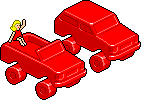
\includegraphics{templatesicon}
\end{figure}


%\chapter{Application Example}

\begin{figure}[htbp]
    \centering

\includegraphics{applicationicon}
\end{figure}



\end{document}